\definecolor{dkgreen}{rgb}{0,0.6,0}
\definecolor{gray}{rgb}{0.5,0.5,0.5}
\definecolor{mauve}{rgb}{0.58,0,0.82}

\lstset{frame=tb,
  language=Python,
  aboveskip=3mm,
  belowskip=3mm,
  showstringspaces=false,
  columns=flexible,
  basicstyle={\small\ttfamily},
  numbers=none,
  numberstyle=\tiny\color{gray},
  keywordstyle=\color{blue},
  commentstyle=\color{dkgreen},
  stringstyle=\color{mauve},
  breaklines=true,
  breakatwhitespace=true,
  tabsize=3
}


% PART 1: PROBLEM FRAMING
\chapter{PROBLEM FRAMING}
\section{Problem Description}
Securing documents—whether physical or digital—remains a persistent, multi-dimensional problem that affects governments, enterprises, and individuals.

\textbf{Physical Documents:} Physical records (e.g., passports, certificates, contracts) have long been protected via signatures, seals, stamps, and locked storage, yet they remain vulnerable to forgery, misuse, and destruction (Figure \ref{signature-forgery}). Law-enforcement bodies warn that advances in consumer printing and imaging have lowered the barrier to document counterfeiting \cite{interpol_identity_nodate}. Border and customs activity shows the problem is active and measurable: in one U.S. port alone, officials intercepted more than 6,800 fraudulent or stolen documents in FY2023—a 219\% year-over-year increase—demonstrating both scale and growth \cite{us_customs_and_border_protection_cincinnati_nodate}. In addition to fraud, disasters can irreparably damage archives; professional guidance exists precisely because fires, floods, and collapses have destroyed unique holdings (e.g., the 2009 Cologne City Archive collapse that obliterated a major European archive) \cite{international_council_on_archives_emergency_nodate,geoengineerorg_cologne_nodate}.

\begin{figure}[H]
    \centering
    
\includegraphics[width=18cm]{"images/signature-forgery.jpg"}
    \caption{Signature Forgery Impact on Important Processes}
    \label{signature-forgery}
\end{figure}

\textbf{Digital Documents:} Digitization improved accessibility and scale but introduced remote theft, silent manipulation, mass leakage, and extortion (Figure \ref{man-in-the-middle}). The scale is well documented: Verizon’s 2024 DBIR analyzed 30,458 incidents with 10,626 confirmed breaches, noting increased vulnerability exploitation via web applications \cite{verizon_2024_nodate}. Financial impact remains high: IBM’s 2025 study reports a global average breach cost of USD 4.4M (down from USD 4.88M in 2024, still historically elevated), underscoring that document exposure is expensive even when containment improves \cite{ibm_cost_nodate,ibm_cost_nodate-1}. Ransomware and data-theft extortion continue to pressure organizations across critical sectors, with complaints to the FBI’s IC3 rising 9\% in 2024 and losses hitting \$16.6B across cyber and scam crimes \cite{reuters__fbi_complaints_nodate}.

\begin{figure}[H]
    \centering
    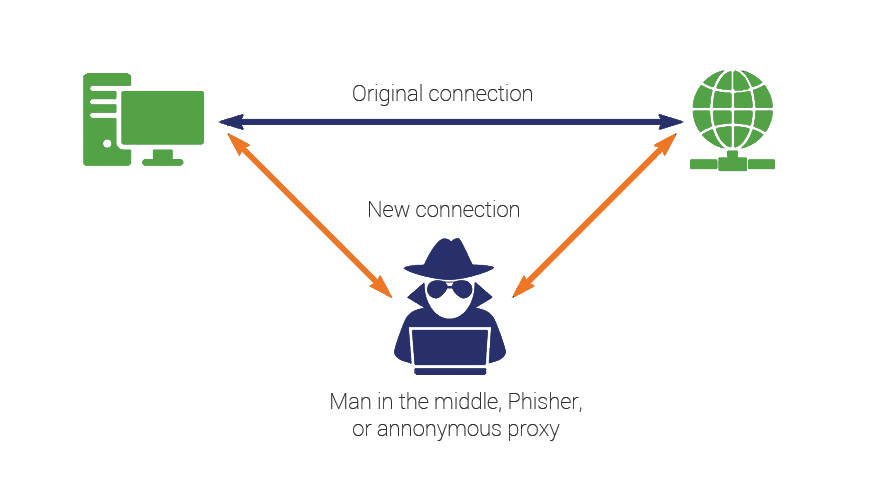
\includegraphics[width=18cm]{"images/man-in-the-middle.png"}
    \caption{Man In The Middle Attack}
    \label{man-in-the-middle}
\end{figure}

\textbf{Trust and authenticity weaknesses in current ecosystems:} Even when digital signatures and PKI are used, centralized trust anchors can fail. The DigiNotar breach (2011) led to hundreds of fraudulent certificates for prominent domains, breaking the authenticity guarantees expected from TLS/PKI and forcing browser vendors to distrust the CA entirely—an instructive “single point of failure” for trust \cite{wired_diginotar_nodate}. The episode shows that document authenticity that depends on a compromised authority can be globally undermined.

\textbf{Human and process error remain a major source of breaches:} Beyond external attackers, misconfigurations, errors, and insider misuse contribute materially to breaches. Verizon’s 2024 DBIR details the role of internal actors and errors across sectors; in healthcare, for example, internal actors feature far more prominently than elsewhere, reversing earlier trends \cite{hipaa_journal_verizon_nodate}. This reflects a broad, persistent problem: authorized access used improperly can compromise sensitive documents at scale.

\textbf{Regulatory pressure - confidentiality, integrity, accountability:} Regulatory frameworks require clear safeguards for documents that include personal data. The GDPR mandates “appropriate technical and organizational measures” and emphasizes data integrity and accountability \cite{eur-lex_gdpr_nodate}. In the EU, eIDAS sets legal scaffolding for electronic identification and trust services, defining requirements for trustworthy digital interactions (e.g., signatures, seals, timestamps) \cite{eur-lex_eidas_nodate}. Non-compliance introduces legal and financial risks on top of the technical ones.

\textbf{Common vulnerability patterns in applications that handle documents:} Applications that store, view, transfer, or sign documents routinely exhibit high-impact weaknesses. The OWASP Top 10 highlights recurring problems such as Broken Access Control (ranked \#1 in 2021), Cryptographic Failures, Injection, and Security Misconfiguration (Figure \ref{owasp-top10}); notably, 94\% of tested apps exhibited some form of access control weakness in the dataset behind the 2021 list \cite{owasp_top_nodate,owasp_a01_nodate}. These patterns map directly to risks for document confidentiality, integrity, and availability.

\begin{figure}[H]
    \centering
    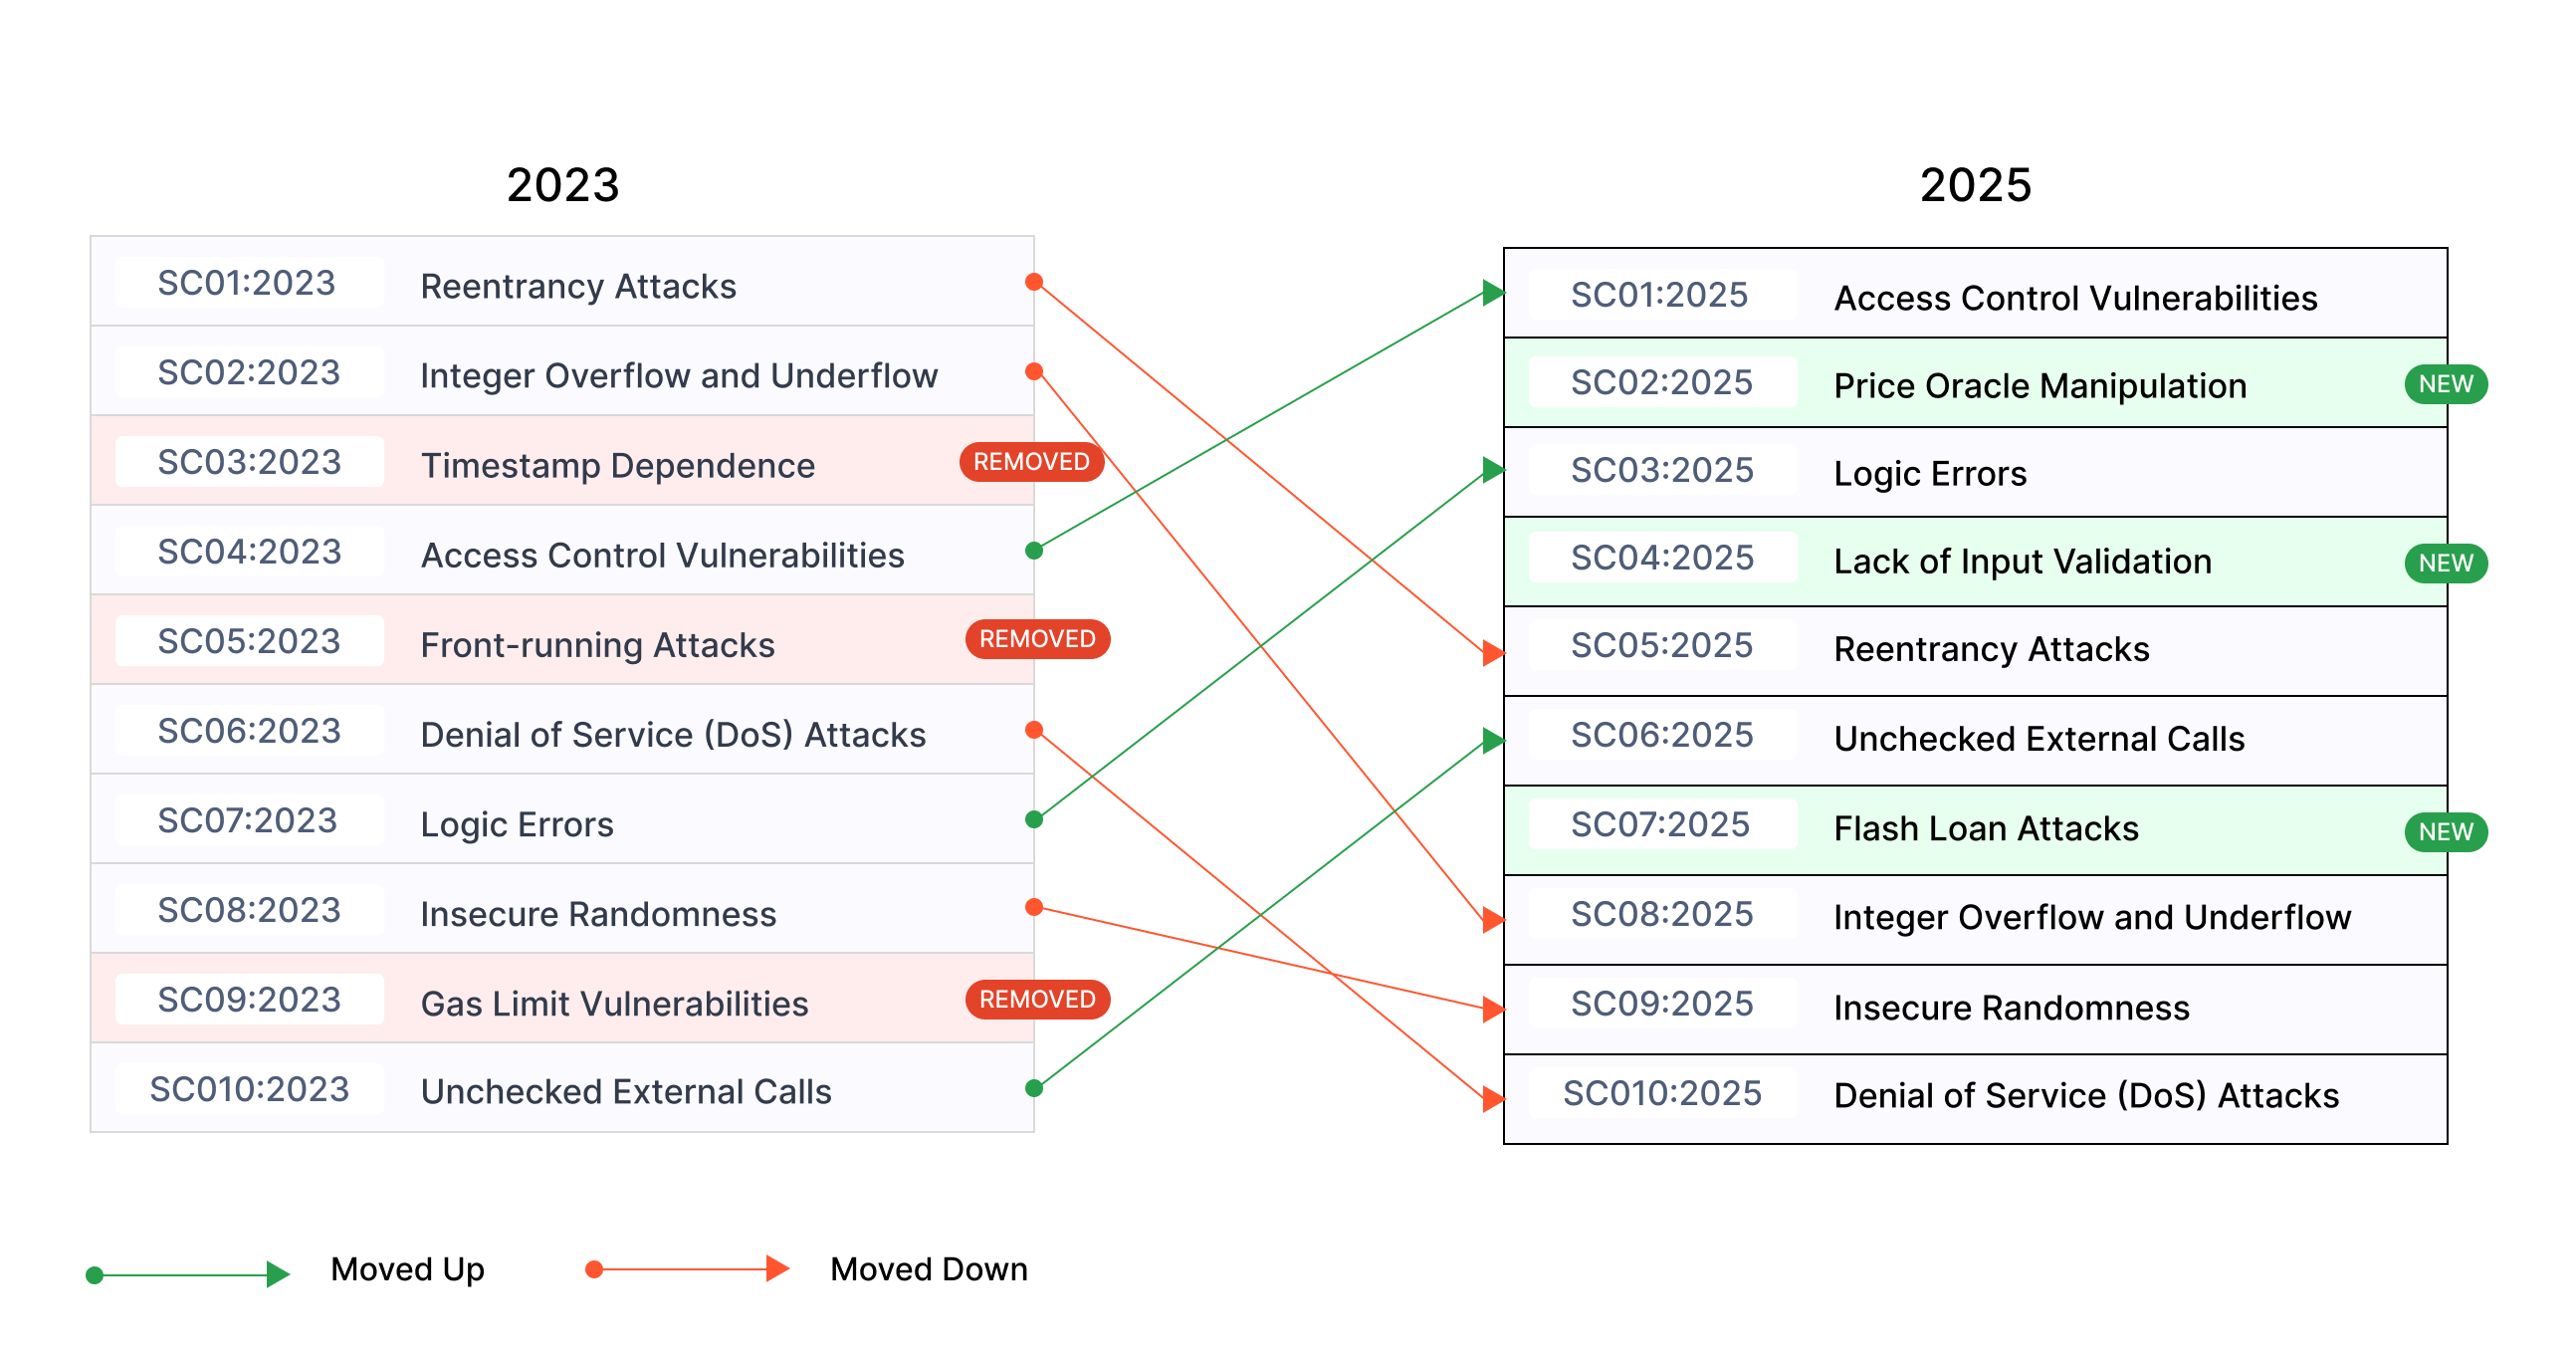
\includegraphics[width=18cm]{"images/owasp-top10.png"}
    \caption{OWASP Top 10 (2023 vs 2025)}
    \label{owasp-top10}
\end{figure}

\textbf{The Core Problem:} Taken together, these issues demonstrate that document security is a multifaceted challenge:

\begin{itemize}
    \item Physical documents face forgery and catastrophic loss risks despite traditional controls \cite{interpol_identity_nodate,us_customs_and_border_protection_cincinnati_nodate,international_council_on_archives_emergency_nodate,geoengineerorg_cologne_nodate}.
    \item Digital documents face breach, extortion, and manipulation at global scale, with material financial impact \cite{verizon_2024_nodate,ibm_cost_nodate,ibm_cost_nodate-1,reuters__fbi_complaints_nodate}.
    \item Trust infrastructures (e.g., CAs) can become single points of failure \cite{wired_diginotar_nodate}.
    \item Human/organizational errors and app-level vulnerabilities remain prevalent \cite{hipaa_journal_verizon_nodate,owasp_top_nodate,owasp_a01_nodate}.
    \item Regulatory frameworks demand provable safeguards and accountability \cite{eur-lex_gdpr_nodate,eur-lex_eidas_nodate}.
\end{itemize}

These facts collectively demonstrate that ensuring authenticity, integrity, confidentiality, availability, and accountability for documents is an unresolved, real-world problem spanning both physical and digital realms.


\section{Problem Statement}
Existing mechanisms for securing physical and digital documents remain vulnerable to forgery, loss, unauthorized access, manipulation, and systemic trust failures, while regulatory obligations require stronger assurance and accountability. The problem is to guarantee authenticity, integrity, confidentiality, availability, and verifiability of documents over time and across domains, despite evolving threats, human error, and infrastructural weaknesses (Figure \ref{soc-compliance-standards}).

\begin{figure}[H]
    \centering
    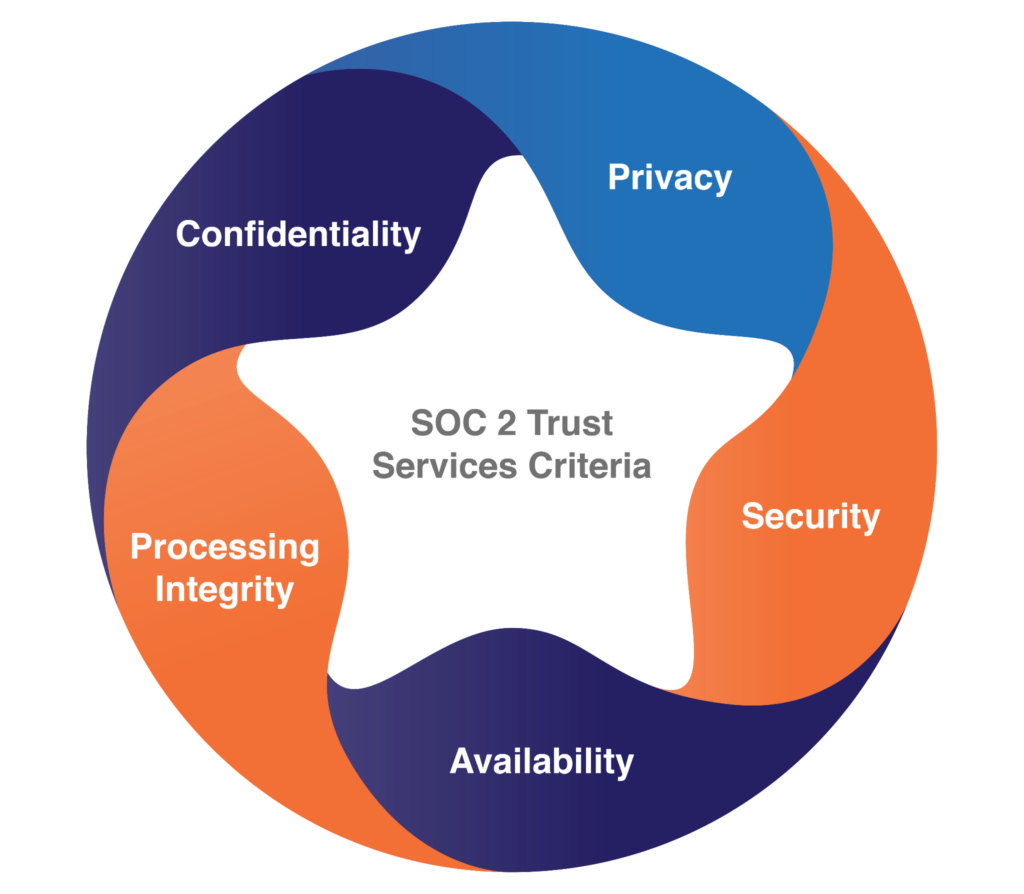
\includegraphics[width=18cm]{"images/soc-compliance-standards.png"}
    \caption{Service Organization Controls (SOC) security principles standard}
    \label{soc-compliance-standards}
\end{figure}


% PART 2: Domain Analysis
\chapter{Domain Analysis}
\section{Target Audience}
BlockSign is designed to serve a diverse range of users who require secure, verifiable, and legally recognized methods of document handling. By leveraging blockchain technology, BlockSign ensures authenticity, immutability, and compliance across various sectors. The primary audiences are described in this section.

\subsection{Individual Users}
In an era where personal data misuse and identity theft are prevalent, individuals can utilize BlockSign to notarize personal documents such as wills, rental agreements, and contracts. This ensures their documents remain immutable and verifiable over time, providing peace of mind and legal assurance \cite{world_economic_forum_global_nodate}.

\subsection{Educational Institutions} 
Educational institutions require secure systems for managing sensitive records, including diplomas, transcripts, and certificates (Figure \ref{digital-certificates}). Cases of diploma fraud have  increased globally, undermining student mobility and employer trust. Blockchain notarization of educational credentials ensures their authenticity across borders, which  is particularly important in student exchange programs and international hiring \cite{unesco_credentials_nodate}.

\begin{figure}[H]
    \centering
    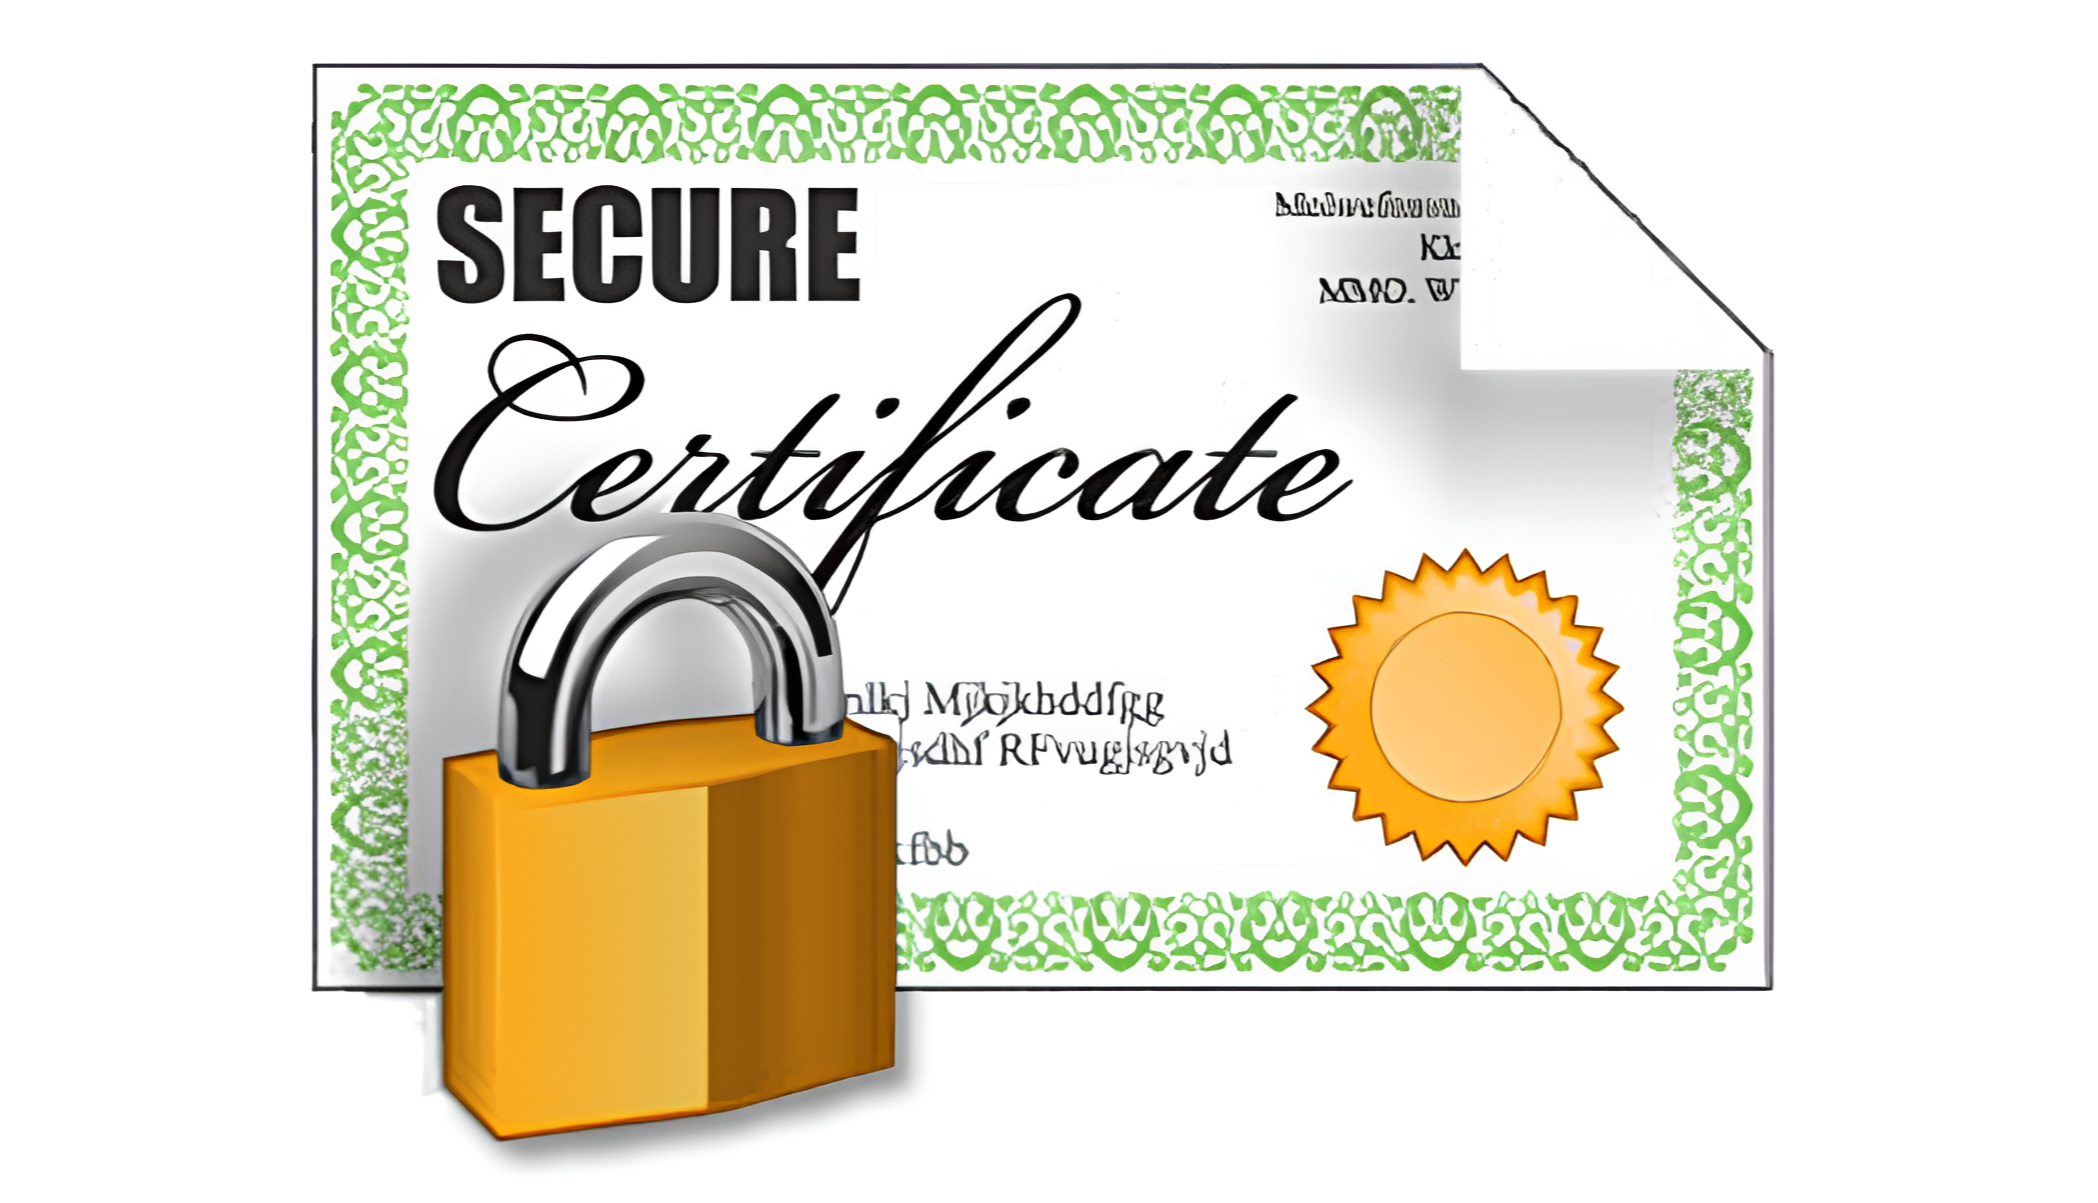
\includegraphics[width=18cm]{"images/digital-certificates.png"}
    \caption{Digital Certificates}
    \label{digital-certificates}
\end{figure}

\subsection{Small and Medium Enterprises (SMEs)} 
SMEs often lack access to enterprise-grade solutions like DocuSign or Adobe Sign due  to cost constraints. BlockSign offers a cost-effective and transparent notarization platform, enabling startups, freelancers, and growing firms to establish trust with partners, clients, and regulators without heavy infrastructure investments \cite{european_comission_digital_nodate}. 

\subsection{Government Institutions} 
Government agencies responsible for issuing and verifying official records (e.g., passports, permits, licenses) face persistent threats from forgery and manipulation of physical and digital documents (Figure \ref{cbp-travel-document}). These institutions require trustworthy digital notarization solutions to comply with regulations such as the EU’s eIDAS Regulation and the General Data Protection Regulation (GDPR) \cite{european_comission_eidas_nodate}. 

\begin{figure}[H]
    \centering
    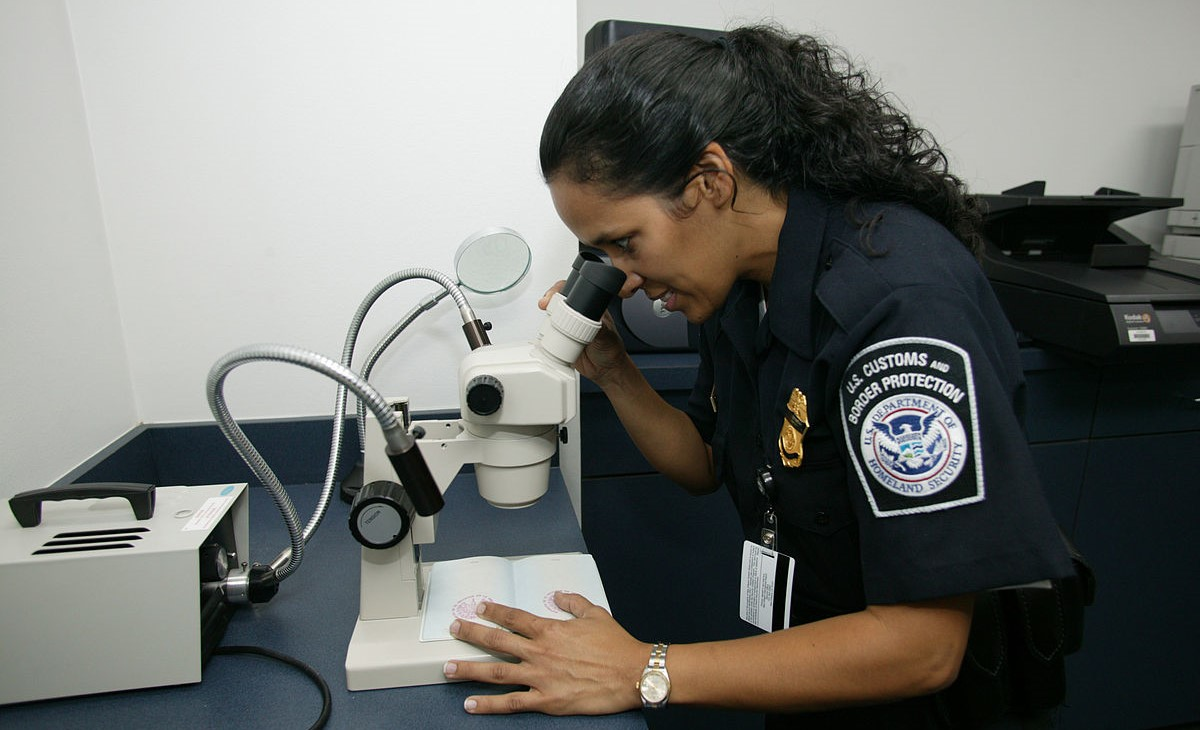
\includegraphics[width=18cm]{"images/cbp-travel-document.jpg"}
    \caption{Customs and Border Protection officer verifying a travel document}
    \label{cbp-travel-document}
\end{figure}

\subsection{Law Firms and Notary Services} 
Law firms and notary services handle contracts, affidavits, and property transactions, all of which require high trust and legal enforceability. Traditional notarization can be time-consuming and limited by geographic restrictions. Remote Online Notarization (RON), already gaining traction in the United States and parts of Europe, demonstrates  that secure video-based validation combined with blockchain immutability can 
streamline legal workflows while retaining compliance \cite{ncfa_canada_future_nodate}. 

\subsection{Financial and Banking Sectors} 
Financial institutions, including banks and insurance companies, must guarantee the  validity of signed contracts, loan agreements, and client identities (Figure \ref{loan-agreement}). Financial institutions are among the industries with the highest breach costs, averaging USD 4.44 million per incident \cite{accenture_state_nodate}.

\begin{figure}[H]
    \centering
    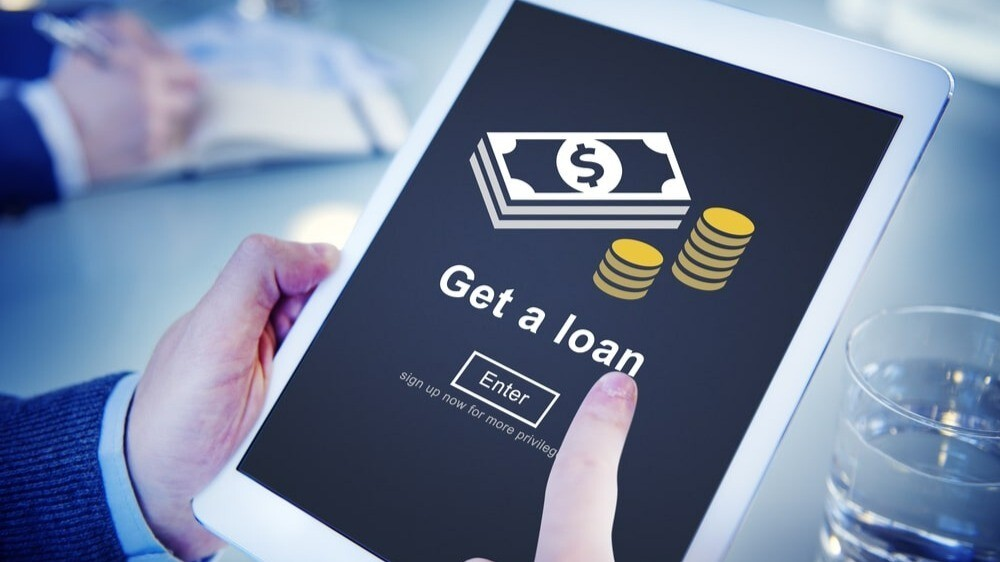
\includegraphics[width=18cm]{"images/loan-agreement.jpg"}
    \caption{Personal Loan Agreement}
    \label{loan-agreement}
\end{figure}

\subsection{Healthcare Organizations} 
The healthcare sector is increasingly dependent on electronic records and digital  consent forms. The sector faces both internal and external threats: 70\% of healthcare  breaches involve insiders misusing access privileges \cite{kadir_canoz_use_nodate}. For hospitals, clinics, and research institutions, BlockSign offers a mechanism to notarize patient records, safeguard sensitive data, and ensure compliance with confidentiality obligations under GDPR. 


\section{Market Size and Growth}
According to industry reports, the global market for digital signatures was worth about USD 7.47 billion in 2023, and it’s expected to soar to around USD 37.79 billion by 2029, expanding at an annual growth rate of 31\%. 

Other estimates are even more bullish: one study puts the 2023 market at USD 4.6 billion with a forecast to USD 43.5 billion by 2030, representing a 37.9\% CAGR between 2023 and 2030 (Figure \ref{market-growth}) \cite{grand_view_horizon_global_nodate}. Another source projects growth from USD 3.2 billion in 2021 to USD 48.4 billion by 2028, at 35.4\% CAGR (Figure \ref{market-growth-2}) \cite{acumen_digital_nodate}. Despite slight variations in numbers, the consensus is clear: the market is booming.

\begin{figure}[H]
    \centering
    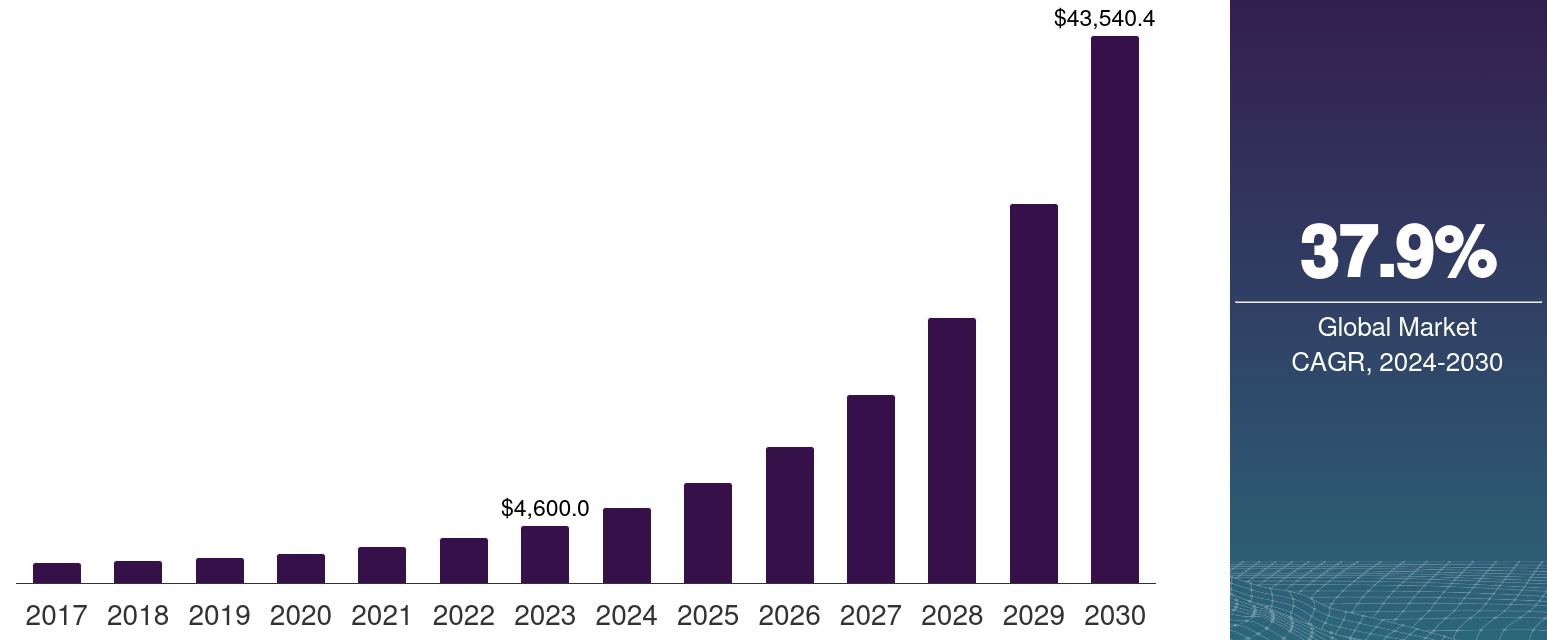
\includegraphics[width=18cm]{images/market-growth.png}
    \caption{Global Digital Signature Market Size 2017-2030 (Horizon)}
    \label{market-growth}
\end{figure}

Blockchain-related identity services and notarization tools are also on the rise, particularly in industries where trust, compliance, and speed are critical: banking, finance, legal, and healthcare. These solutions help reduce fraud, accelerate cross-border processes, and ensure compliance with regulations like GDPR, eIDAS in Europe, or ESIGN and UETA in the United States.

\begin{figure}[H]
    \centering
    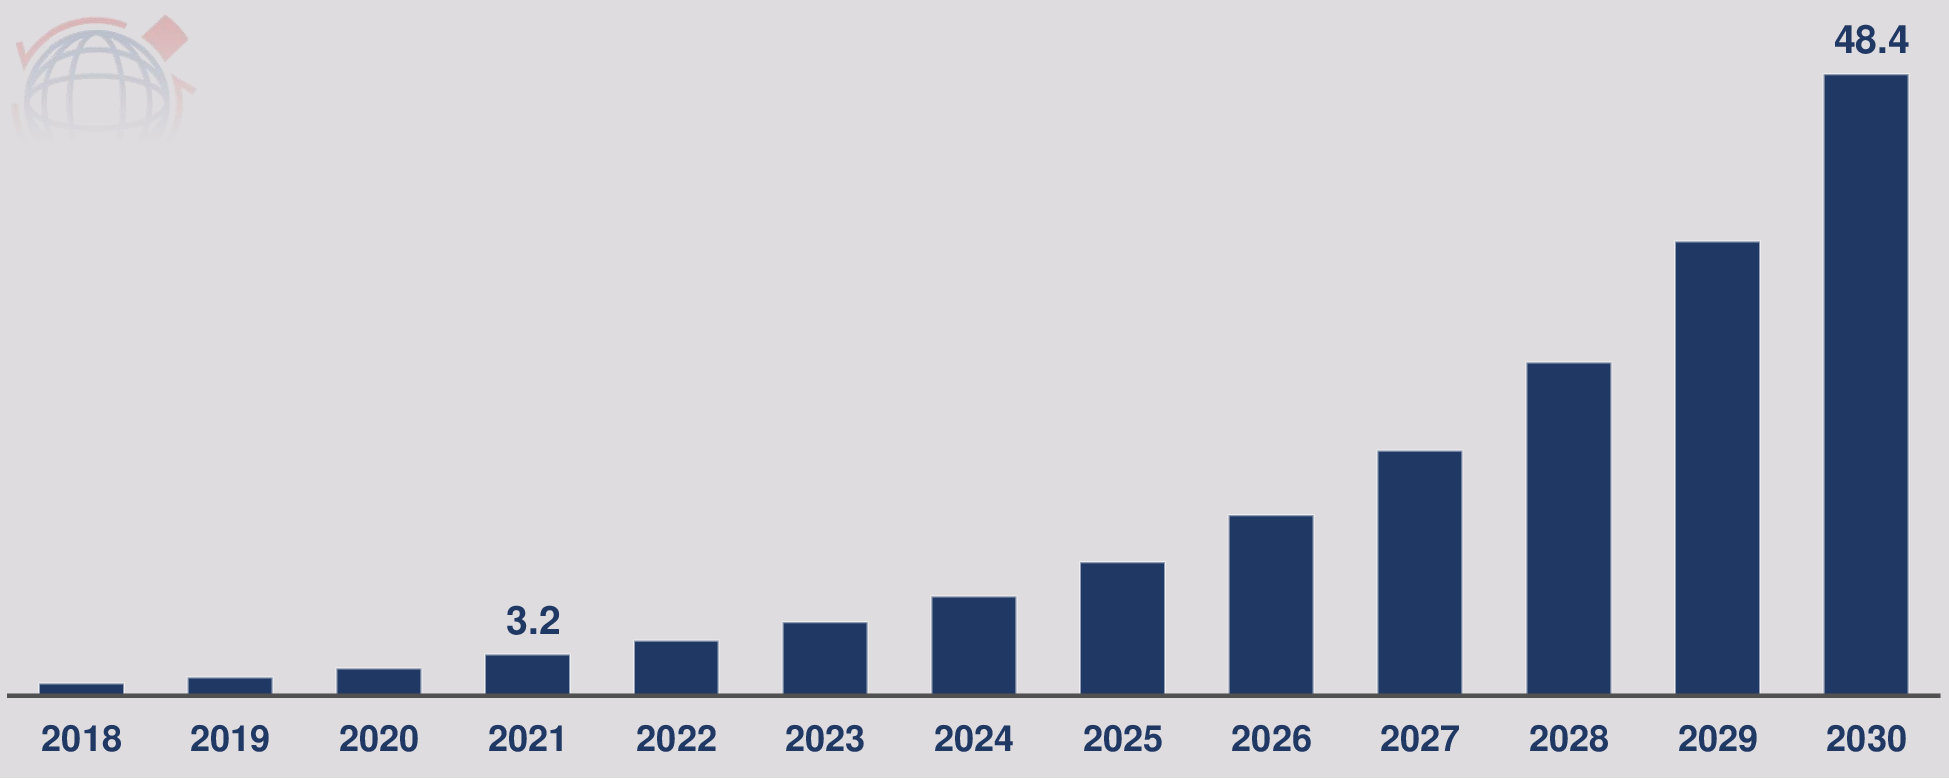
\includegraphics[width=18cm]{images/market-growth-2.png}
    \caption{Digital Signature Market 2018-2030 (Acumen)}
    \label{market-growth-2}
\end{figure}

\subsection{Key Competitors and Solutions}
Several big players are driving the digital signature space:

\begin{itemize}
    \item \textbf{DocuSign} and \textbf{Adobe Sign} are trusted and widely used, especially by enterprises, but still rely on centralized infrastructure.
    \item \textbf{Notarize}, \textbf{NotaryCam}, and \textbf{SignNow} specialize in Remote Online Notarization (RON), often using video identity checks to meet legal and compliance needs.
    \item On the blockchain side, platforms like \textbf{DoxyChain} and \textbf{Blocknotary} offer immutable timestamping and decentralized storage.
    \item Emerging frameworks like \textbf{KILT Protocol} and \textbf{Concordium} support decentralized identity and can integrate into notarization workflows.
\end{itemize}

These players show how mature the e-signature market is becoming—and how blockchain is carving out its place as a serious value-add technology (Figure \ref{market-share}) \cite{electro_iq_e-signature_nodate}.

\begin{figure}[H]
    \centering
    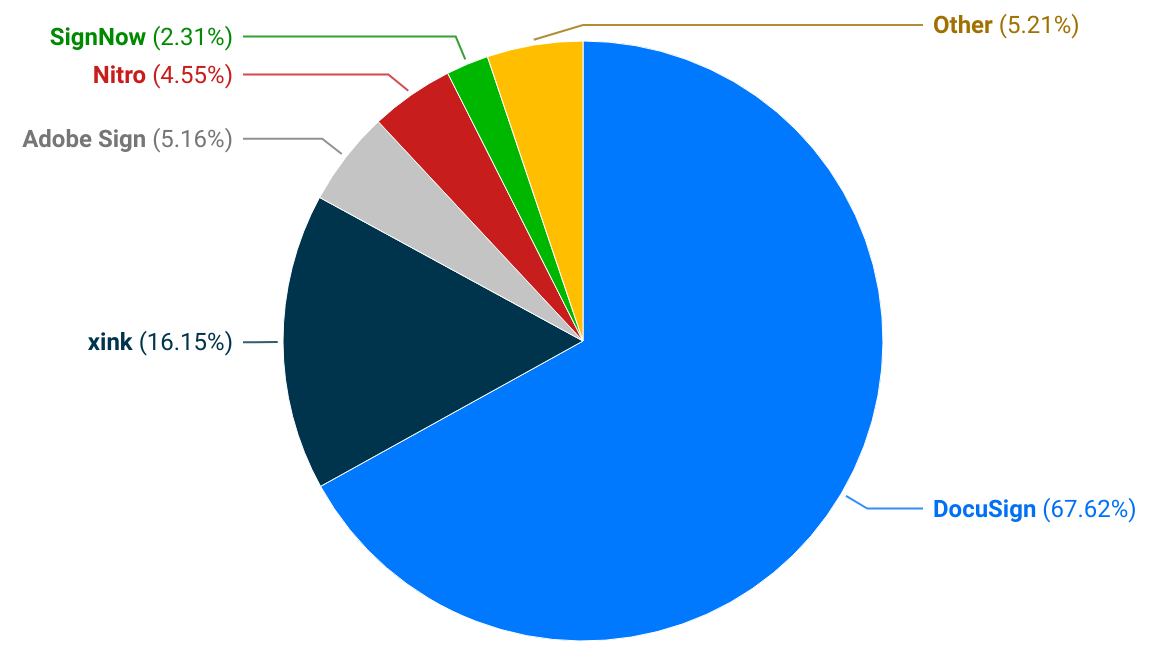
\includegraphics[width=18cm]{images/market-share.png}
    \caption{Market Share of Leading Electronic Signature Companies}
    \label{market-share}
\end{figure}

\subsection{Trends and Opportunities}
A few clear trends are shaping the future of digital signatures:

\begin{enumerate}
    \item \textbf{Trustless, decentralized verification} – Blockchain-based notarization helps remove single points of failure tied to central Certificate Authorities (CAs).
    \item \textbf{Remote and cross-border notarization} – With more people working globally, demand increases for legally recognized remote notarization systems.
    \item \textbf{AI and automation integration} – Automated document checks, fraud detection, and smart contract workflows are on the rise.
    \item \textbf{Quantum-safe cryptography} – Some platforms are starting to prepare for future cryptographic threats to ensure long-term document integrity.
    \item \textbf{Hybrid architectures} – Combining public and permissioned blockchains helps balance trust, scalability, and cost-efficiency.
\end{enumerate}

These trends create fertile ground for innovation, especially for solutions that balance security, legal compliance, and user-friendliness (Figure \ref{benefits-signatures}).

\begin{figure}[H]
    \centering
    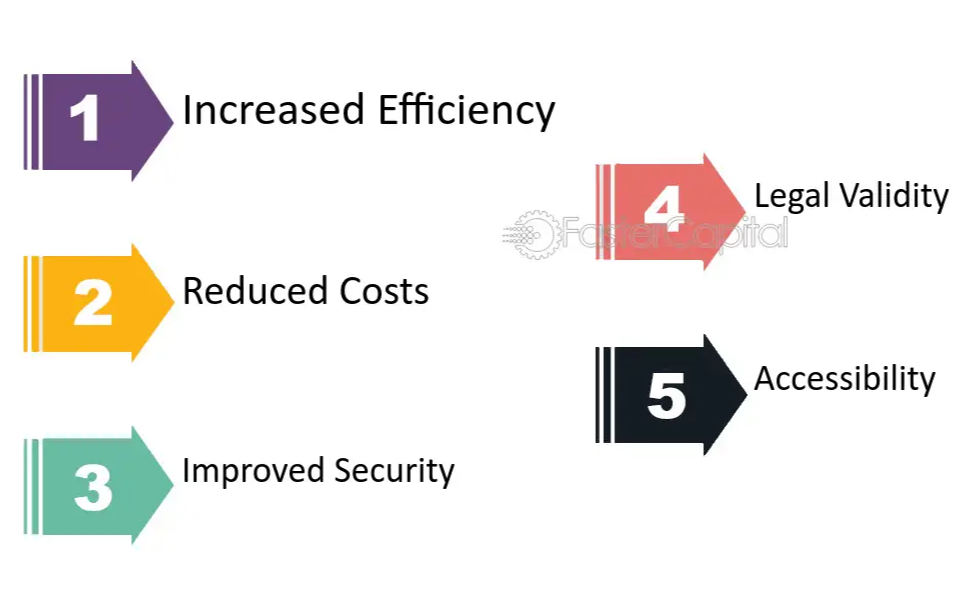
\includegraphics[width=18cm]{images/benefits-signatures.png}
    \caption{Benefits of Digital Signatures}
    \label{benefits-signatures}
\end{figure}

\subsection{Challenges and Barriers}
However, adoption still faces some challenges:

\begin{itemize}[leftmargin=1.5em]
    \item Legal frameworks vary widely across countries, slowing global standardization and interoperability.
    \item Many institutions remain comfortable with traditional notarization; change can feel risky.
    \item Balancing high security with simplicity is tough—systems that are too complex won’t encourage adoption.
    \item Public blockchains can struggle with scalability and can be costly for frequent use.
\end{itemize}


\section{Technical Research}
This section describes core technologies potentially applicable for implementing the secure document notarization idea. For each, it will be described how it operates, its benefits, and real-world usage.

\subsection{Blockchain-Based Notarization}
Document notarization on blockchain typically involves computing a cryptographic hash of the file and storing it timestamped on a decentralized ledger. Anyone can later rehash the document to verify integrity without revealing the document’s content \cite{doxychain_power_nodate}. Some valuable benefits of this approach are:

\begin{itemize}
    \item \textbf{Immutability and transparency:} Hash entries cannot be altered after being written to the chain and are visible across the network (Figure \ref{blockchain-notarization}).
    \item \textbf{No central point of failure:} Decentralized consensus removes reliance on a single trusted authority \cite{deeksha_uikey_blockchain-based_nodate}.
    \item \textbf{Timeproof:} Timestamps on transactions provide verifiable evidence of document existence at a given time \cite{doxychain_power_nodate}.
\end{itemize}

\begin{figure}[H]
    \centering
    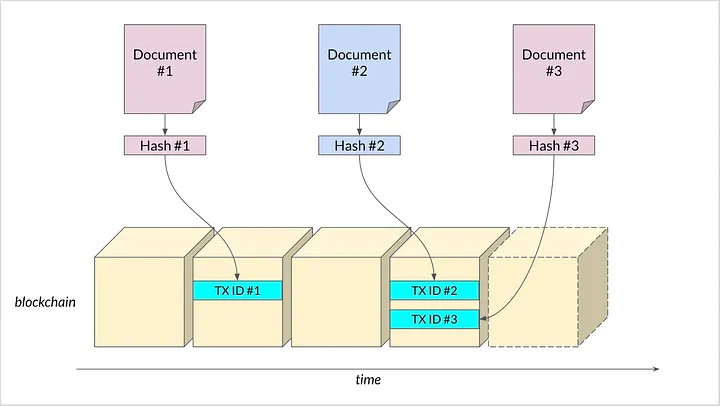
\includegraphics[width=18cm]{"images/blockchain-notarization.png"}
    \caption{Blockchain Notarization}
    \label{blockchain-notarization}
\end{figure}

Recent academic research explores moving from simple “proof of existence” to full document validation, integrating smart contracts, Zero-Knowledge Proofs (ZKPs), AI-based content analysis, and quantum-resistant cryptography—to ensure privacy, detect fraud, and future-proof security \cite{tejas_chandrakant_mhapankar_future_nodate}. Hybrid blockchain architectures are also being proposed to improve scalability and cost-efficiency, balancing public and permissioned ledger benefits \cite{domenico_tortola_scalable_nodate}.

\subsection{Electronic Signatures with Multi-Factor Authentication}
Combining digital signatures with MFA requires users to authenticate via multiple channels—e.g., password plus a one-time code or biometric—before signing or notarizing a document (Figure \ref{multifactor-auth}) \cite{sutisoft_role_nodate}. Several useful features and benefits are:

\begin{itemize}
    \item \textbf{Significantly enhanced security:} Microsoft reports that MFA can block 99.2\% of account compromise attacks \cite{pingidentity_eight_nodate}.
    \item \textbf{Fraud reduction:} Additional authentication steps make forging or stealing identities substantially harder \cite{sutisoft_role_nodate,uplevel_systems_top_nodate}.
    \item \textbf{Regulatory compliance:} MFA aids in meeting stringent identity verification requirements in sectors like finance and legal services \cite{sutisoft_role_nodate}.
\end{itemize}

\begin{figure}[H]
    \centering
    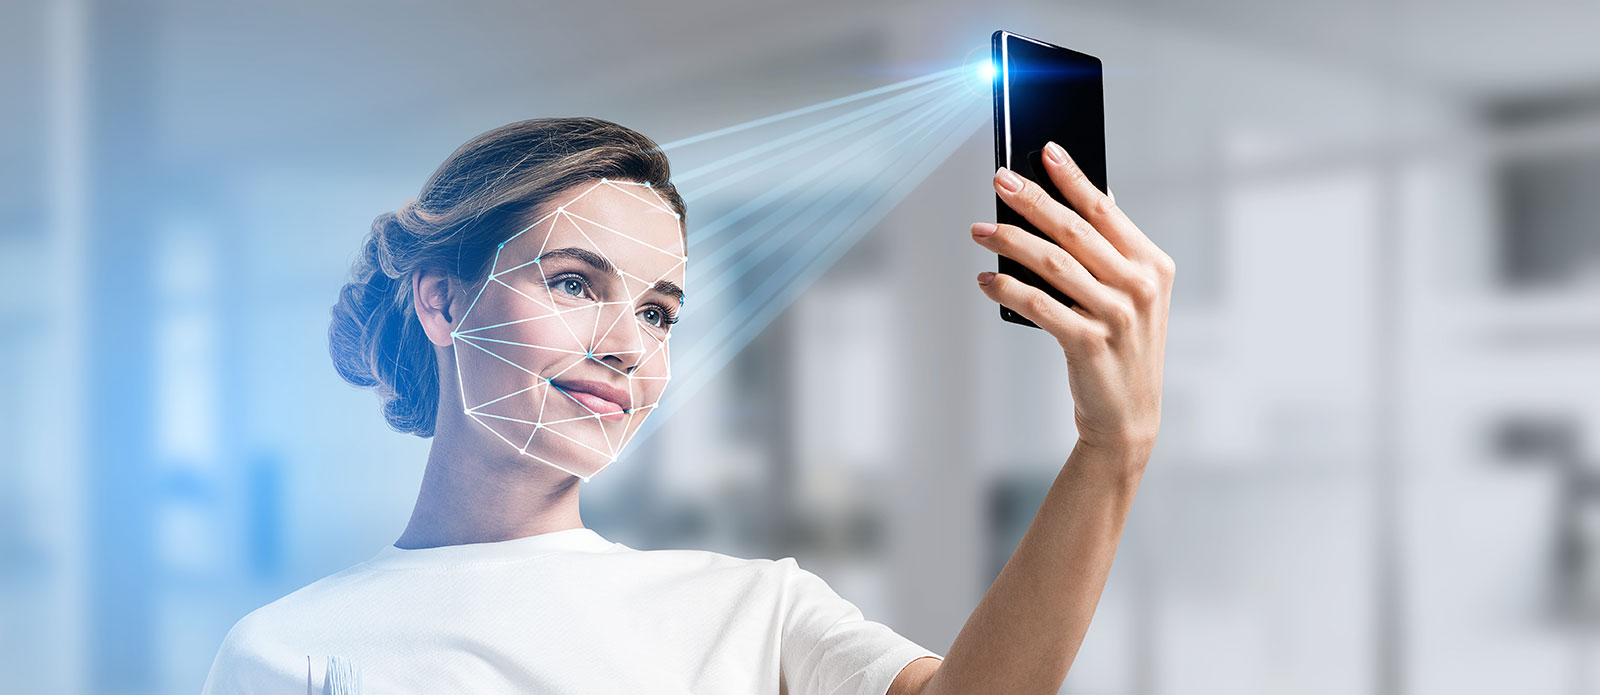
\includegraphics[width=18cm]{"images/multifactor-auth.jpg"}
    \caption{Multi-Factor Authentication}
    \label{multifactor-auth}
\end{figure}

Remote Online Notarization (RON) platforms integrate MFA to verify signer identity and prevent unauthorized access—combining this with tamper-evident seals and audit trails strengthens legal validity and trust \cite{pronotary_how_nodate}.

\subsection{Electronic \& Remote Notarization}
E-Notary systems use digital signatures, cryptographic seals, and a public key infrastructure (PKI) to notarize documents electronically. Remote Online Notarization (RON) adds a layer of video verification and identity validation via secure video + digital credentialing (Figure \ref{multifactor-auth}) \cite{wikipedia_enotary_nodate}. The benefits include:

\begin{itemize}
    \item \textbf{Tamper-evident documents:} Digital signatures and seals prevent unnoticed alterations.
    \item \textbf{Cost savings and efficiency:} Eliminates paper handling and on-site meetings; notarizations can be completed online, rapidly.
    \item \textbf{Audit trails:} Many systems log each step of the notarization process, boosting transparency and legal compliance.
\end{itemize}

\begin{figure}[H]
    \centering
    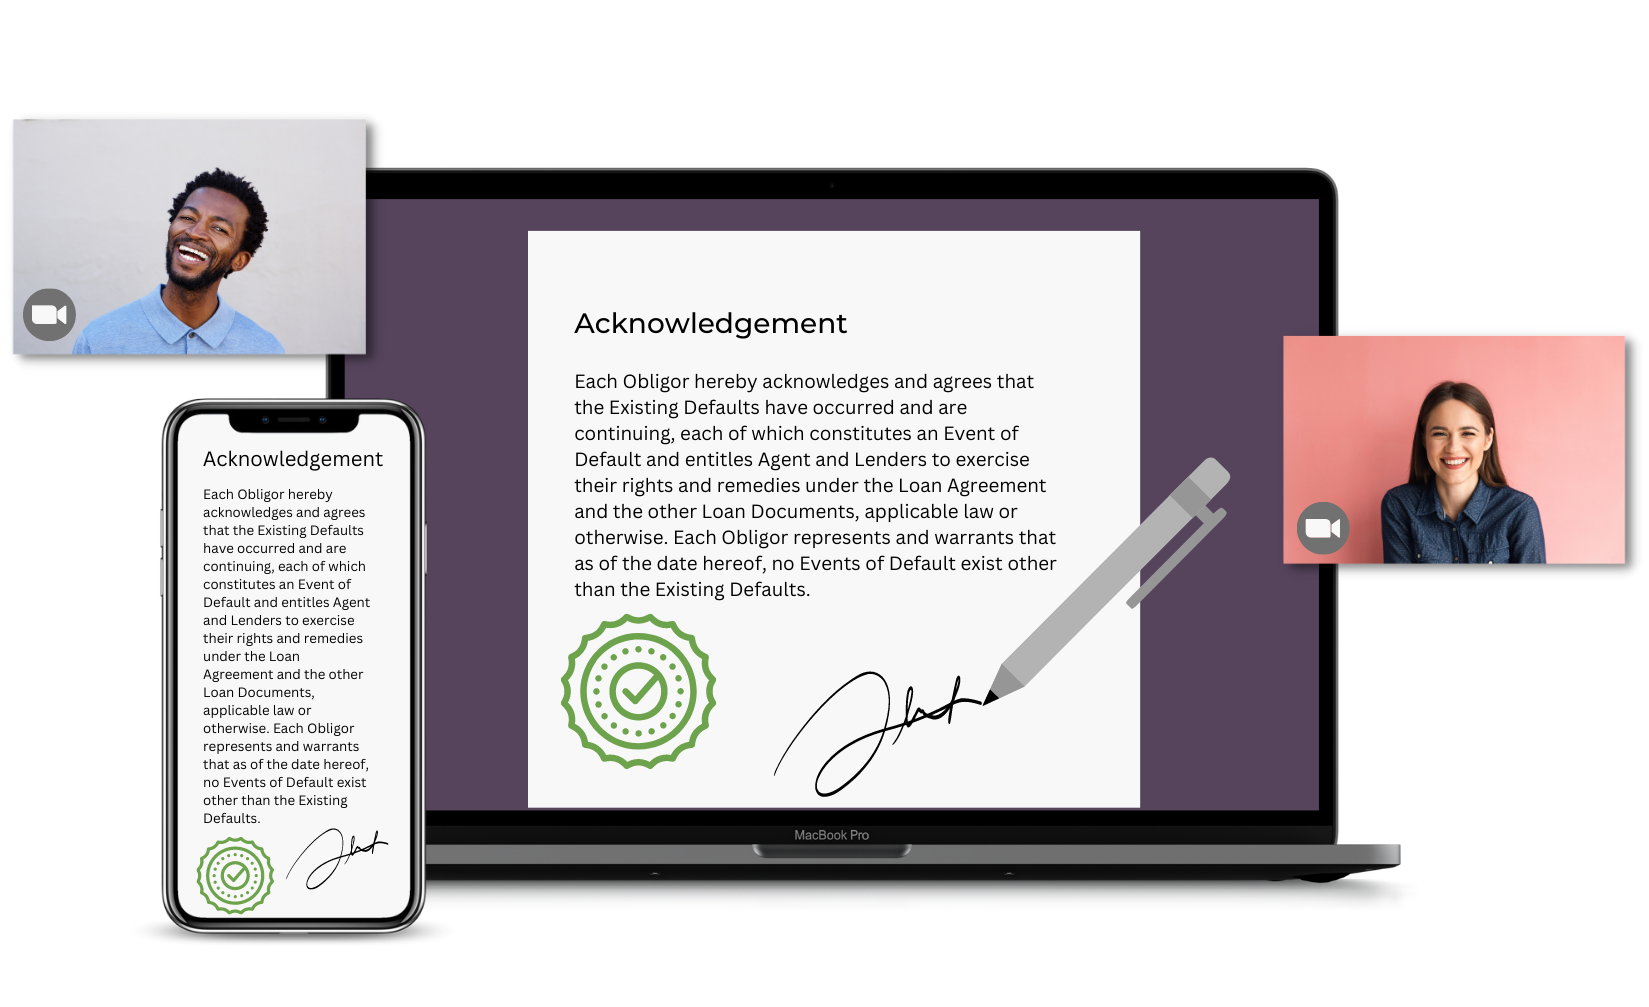
\includegraphics[width=18cm]{"images/remote-notarization.png"}
    \caption{Remote Notarization}
    \label{remote-notarization}
\end{figure}

For example, Notario.org offers an online notarization platform supporting identity verification via video, digital certificates, and legal compliance across several countries (Spain, USA, Germany, etc.) \cite{wikipedia_notario_nodate}.

\subsection{Advanced Cryptographic Techniques}
Zero-Knowledge Proofs (ZKPs) enable one party to prove a statement is true without revealing the underlying data. In blockchain notarization, ZKPs can allow verification of document integrity or content compliance without exposing sensitive data (Figure \ref{multifactor-auth}) \cite{wikipedia_privacy_nodate}. The two benefits of this technique are:

\begin{itemize}
    \item \textbf{Privacy preservation:} Keeps personal or confidential document content hidden while still proving authenticity.
    \item \textbf{Regulatory advantages:} Complies with data protection regulations by limiting exposure of sensitive data.
\end{itemize}

\begin{figure}[H]
    \centering
    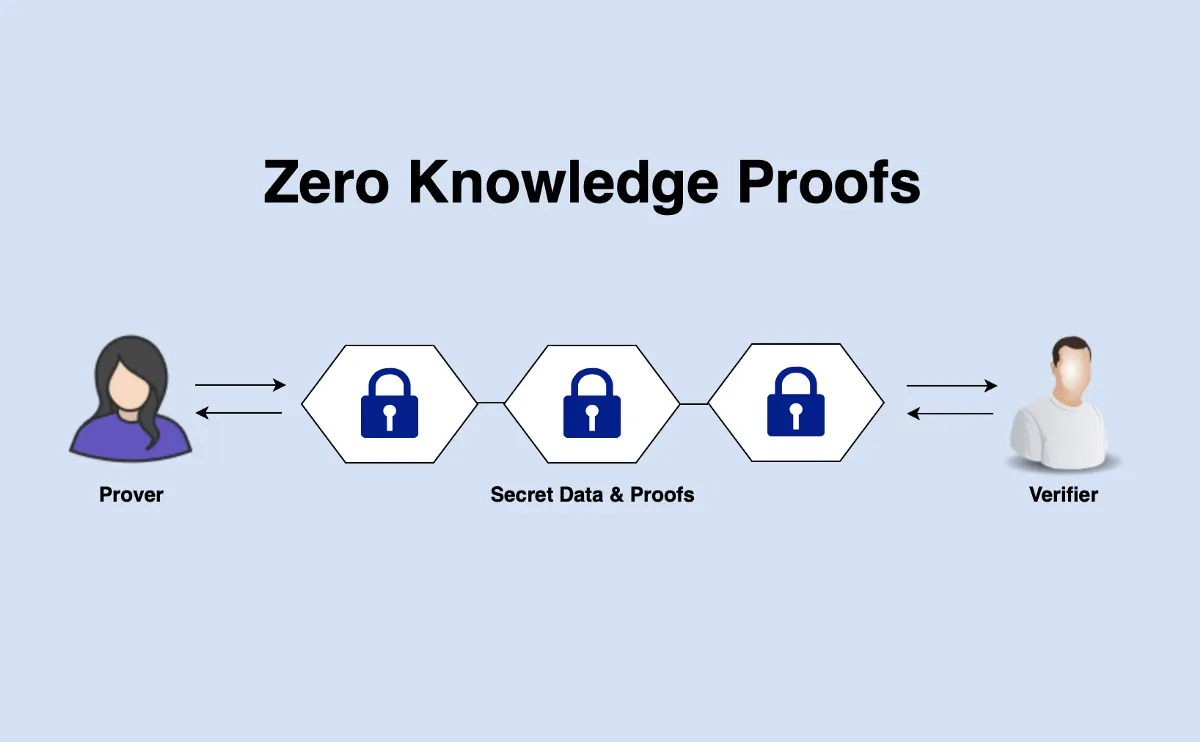
\includegraphics[width=18cm]{"images/zero-knowledge.png"}
    \caption{Zero-Knowledge Proof Mechanism}
    \label{zero-knowledge}
\end{figure}

With the potential arrival of quantum computing, future document notarization systems must adopt quantum-safe cryptographic algorithms to remain secure long-term. Research highlights this as an evolving domain in notarization systems to guard against future computational threats.

\subsection{Hybrid and Scalable Architectures}
To address limitations of public blockchains (e.g., transaction fees, latency) and private blockchains (e.g., trust, centralization), hybrid DLT (Distributed Ledger Technology) designs are emerging. They combine local/private storage for efficiency with public chains for decentralization and transparency. Benefits include:

\begin{itemize}
    \item \textbf{Cost optimization:} Keeps frequent notarizations low-cost by batching hashing operations off-chain while anchoring checkpoints on-chain.
    \item \textbf{Scalability:} Manages large volumes efficiently while maintaining tamper evidence and verifiability.
\end{itemize}


% PART 3: Solution Proposal
\chapter{Solution Proposal}
Based on defined problems and domain research, it is evident that existing document management approaches face serious limitations. Physical records remain vulnerable to forgery, loss, and destruction, while digital records suffer from risks such as unauthorized modification, cyberattacks, and dependence on centralized authorities. Current protections, including digital signatures and certificate-based systems, mitigate some threats but are not sufficient to guarantee authenticity, long-term verifiability, and compliance with modern security standards. At the same time, regulatory frameworks such as GDPR and eIDAS demand solutions that ensure confidentiality, integrity, and accountability. These findings highlight the need for a system that not only secures documents but also provides transparency, privacy, and user trust.

The proposed solution is a blockchain-based notarization platform that enables the creation, signing, and verification of documents in a secure and transparent manner. The platform leverages blockchain to store only the cryptographic hash of documents, ensuring immutability and tamper resistance without exposing sensitive content. This approach allows users to instantly verify document authenticity by comparing a locally computed hash with the one recorded on the blockchain, making the verification process fast, reliable, and independent of intermediaries.

The architecture of the system is structured around four main components:
\begin{enumerate}
    \item \textbf{Client Applications (Web and Mobile)} – provide users with an accessible interface to create, sign, and verify documents. Both platforms support multilingual functionality (English, Russian, Romanian) and integrate usability features such as search, filtering, and history tracking.
    \item Authentication and Identity Management – user authentication is handled through Google OAuth2 and local registration flows, with strong password policies and multi-factor authentication (MFA) applied during sensitive operations such as signing. Identity verification relies on a one-time check of personal identifiers (e.g., IDNP), which are not stored long term, ensuring compliance with privacy regulations. Session management is secured with JWT tokens.
    \item Application Server – coordinates document workflows, including creation, pending approvals, and signature collection. The server computes document hashes, manages participant approvals, and interacts with both the blockchain network and the database. It also enforces security controls such as input validation, secure APIs, and proper session handling.
    \item Blockchain and Database Layer – the blockchain serves as a public, immutable ledger for document hashes, timestamps, and participant references, ensuring integrity and transparency. The database stores only operational metadata and user account information, excluding sensitive identity data. Together, these layers guarantee both system efficiency and data protection.
\end{enumerate}

Functionally, the platform supports a full document lifecycle: registration and identity verification, creation and upload of documents, participant assignment, approval workflows, signing, and final notarization on the blockchain (Figure \ref{signing-verifying}). Each step is backed by security controls, ensuring that fraudulent activity, tampering, or unauthorized access is either prevented or immediately detectable.

\begin{figure}[H]
    \centering
    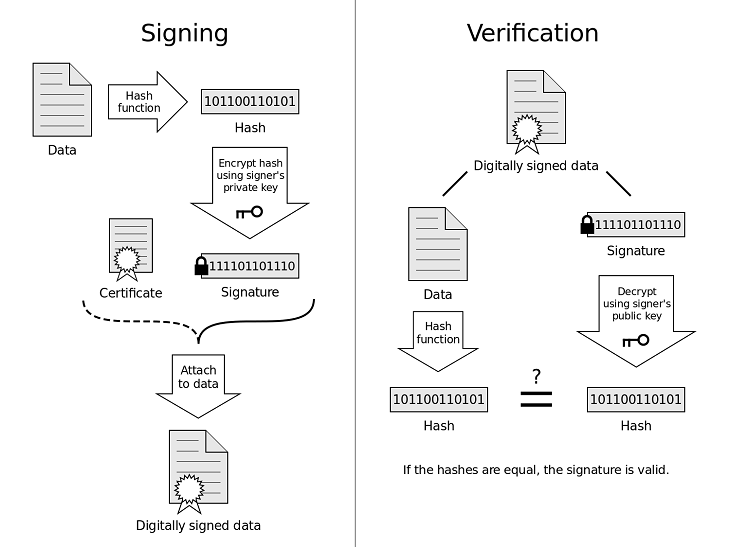
\includegraphics[width=18cm]{"images/signing-verifying.png"}
    \caption{Core Signing and Verifying Logic}
    \label{signing-verifying}
\end{figure}

By combining usability, regulatory compliance, and cryptographic trust mechanisms, the solution directly addresses the shortcomings identified in traditional document management. It provides a system that ensures authenticity, integrity, transparency, and privacy, offering users a verifiable and tamper-proof method of managing critical documents.


% PART 4: System Design
\chapter{System Design}
\section{Technical Requirements}
This section describes the architectural backbone of the project, mainly Functional and Non Functional requirements. It describes key actors, functionalities accessed by them, as well as other technical specifications which will be considered in the project practical implementation part (Figure \ref{func-non-func}). 

\begin{figure}[H]
    \centering
    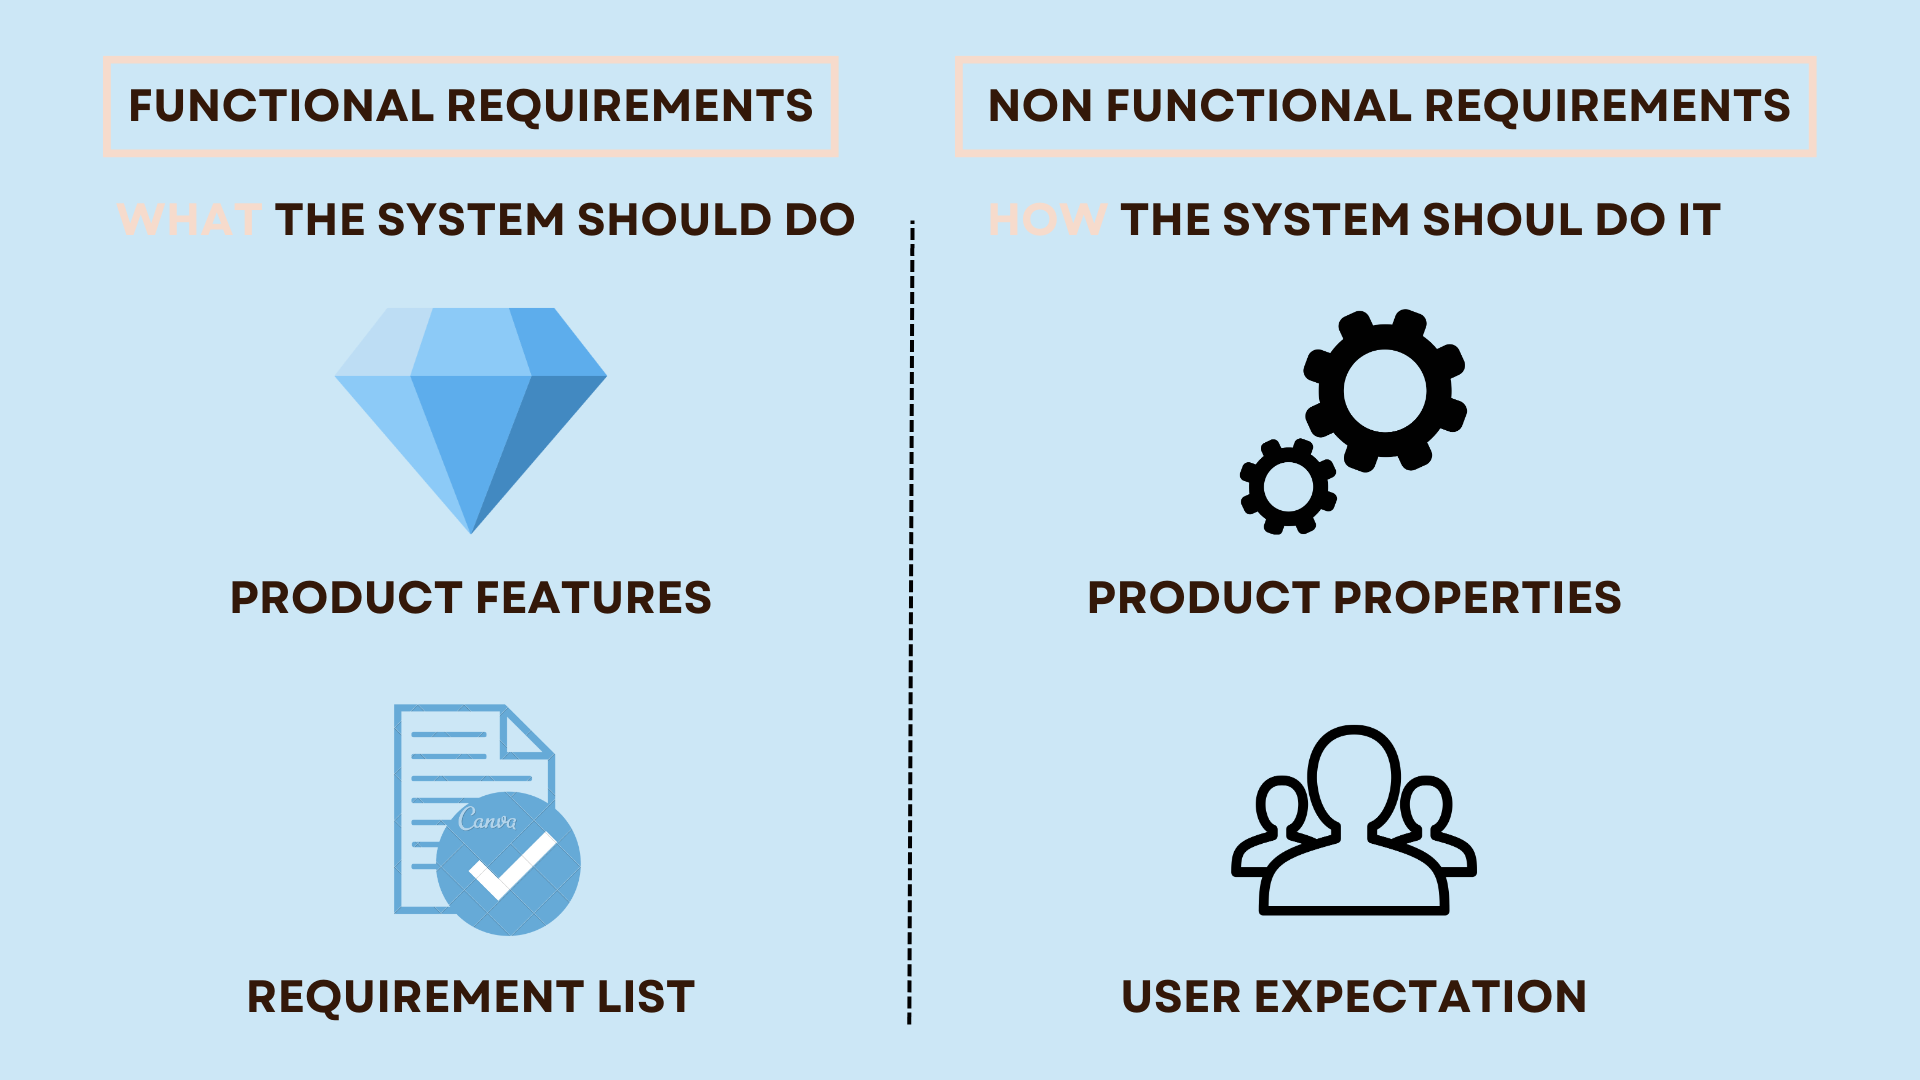
\includegraphics[width=18cm]{"images/func-non-func.png"}
    \caption{Functional And Non-Functional Requirements}
    \label{func-non-func}
\end{figure}

\subsection{Functional Requirements}
The application is designed around three primary user roles:
\begin{enumerate}
    \item \textbf{Unauthorized users}, who may access only the main page and perform registration or login.
    \item \textbf{Authorized users}, who gain full access to document-related services such as creation, signing, verification, and account management.
    \item \textbf{Administrators}, who are responsible for managing the user database and can access limited user information when necessary.
\end{enumerate}

The system incorporates a wide set of functions to support these roles. First, it provides multilingual support, ensuring that the entire interface is available in English, Russian, and Romanian. The main page allows navigation to registration, login, and account pages, as well as a mail integration for sending quick requests to support.

On the documents page, authorized users may create new documents by uploading files through a drag-and-drop interface, specifying the parties involved, and submitting them for signing. Pending documents appear in the personal cabinet of each participant until all signatures are collected. At the same time, users can verify documents by uploading a file, generating its hash, and comparing it with blockchain records. If no match is found, a notification is displayed.

The account page contains a full history of signed and pending documents. Each entry provides a preview, the date, file size, hash, status, and the option to download. Account management includes editing personal details, changing passwords, enabling multi-factor authentication, verifying a phone number, and connecting an authenticator app.

Additional functionality is provided through search and filters, which allow users to locate documents based on keywords, sides, or metadata. Pending documents can be opened in a PDF viewer for review and signed electronically. Once the final party signs, the system hashes the document and records it immutably on the blockchain.

Finally, the system enforces secure authorization and registration flows. Users may authenticate through Google OAuth 2.0 or via local registration (Figure \ref{oauth-mechanism}). 

\begin{figure}[H]
    \centering
    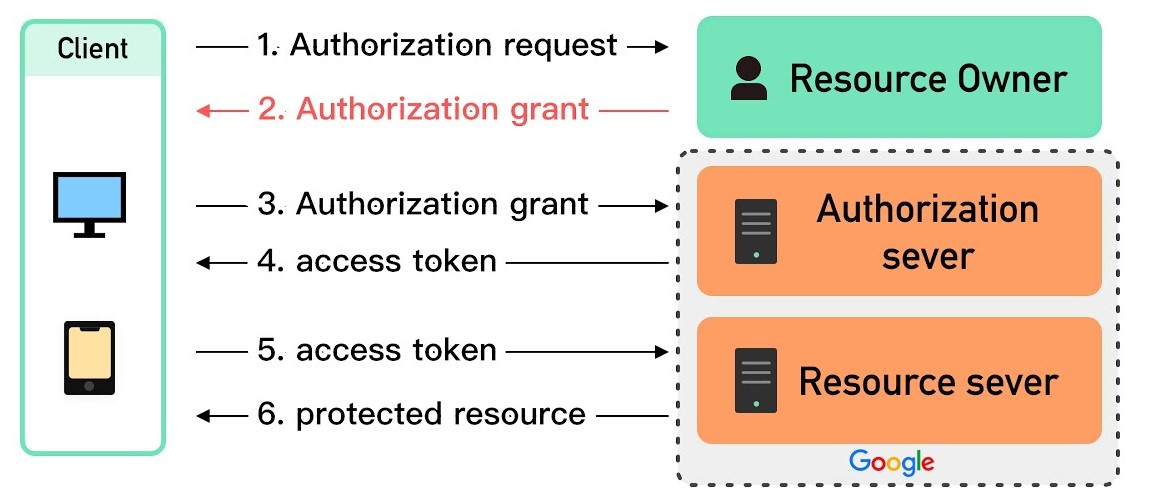
\includegraphics[width=18cm]{"images/oauth-mechanism.jpg"}
    \caption{OAuth Mechanism Description}
    \label{oauth-mechanism}
\end{figure}

Registration follows a structured, multi-step process: (1) account creation with password and phone validation, (2) email verification through a six-digit code, and (3) submission of identity data (IDNP, birth date, selfie) for administrative approval. A password recovery mechanism is also implemented, allowing users to initiate a reset request by email, verify the reset code, and set a new password meeting complexity requirements .

\subsection{Non-Functional Requirements}
Beyond functionality, the application is governed by several non-functional requirements that ensure its performance, usability, and security.

From a performance perspective, documents themselves are never stored on the blockchain. Instead, only their final cryptographic hash is recorded. This guarantees integrity verification without exposing sensitive content or overloading the ledger.

Regarding usability, the system is designed as both a web application and a mobile application, ensuring broad accessibility. To support a diverse user base, the entire interface is available in three languages: English, Russian, and Romanian.

In terms of security, the platform adopts multiple protective measures:
\begin{enumerate}
    \item \textbf{Sensitive data minimization} – personal identifiers such as IDNP are used solely during registration for verification and are not retained long-term.
    \item \textbf{Multi-factor authentication (MFA)} – required for signing documents, adding an extra layer of identity assurance.
    \item \textbf{JWT tokens} – used to secure session management and provide controlled access to the personal cabinet (Figure \ref{jwt-mechanism}).
\end{enumerate}

\begin{figure}[H]
    \centering
    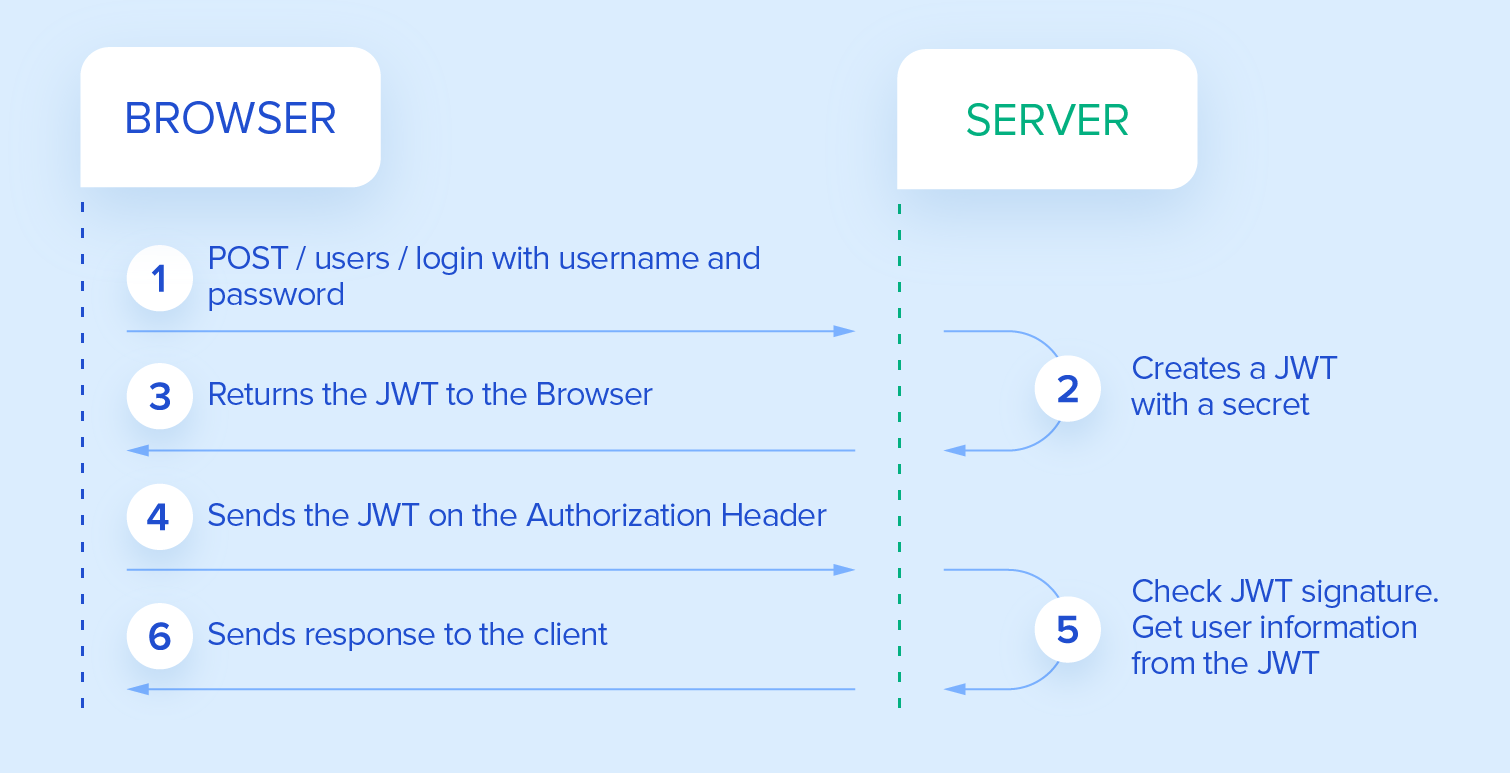
\includegraphics[width=18cm]{"images/jwt-mechanism.png"}
    \caption{JWT Token Usage Mechanism}
    \label{jwt-mechanism}
\end{figure}

Finally, the system adheres to privacy and compliance standards. The blockchain stores only document hashes, with no personal data or file content, ensuring confidentiality and compliance with data protection principles.


\section{Behavioral Modeling}
To capture the dynamic aspects of the system and illustrate how users and components interact, several UML diagrams were created. These diagrams help visualize workflows, user interactions, and message flows between system elements, making the architecture more comprehensible and easier to validate against requirements.

\subsection{Use Case Diagrams}
The use case diagrams represent the primary interactions between different user roles and the system, highlighting the functionalities available to each category of user. There are four main use cases described:
\begin{enumerate}
    \item \textbf{Registration process:} The Figure \ref{uml-use-registration} illustrates the registration process for an unauthenticated user. The actor initiates the flow by selecting the option to register into the system. The process includes several mandatory steps such as filling in registration data, providing personal information, verifying the email, and awaiting administrator approval. An optional extension allows the user to authenticate through Google OAuth as part of the email verification step. The diagram highlights the dependencies between activities using «include» and «extend» relationships, showing that registration is a structured, multi-step procedure designed to ensure security and identity verification.
    \begin{figure}[H]
        \centering
        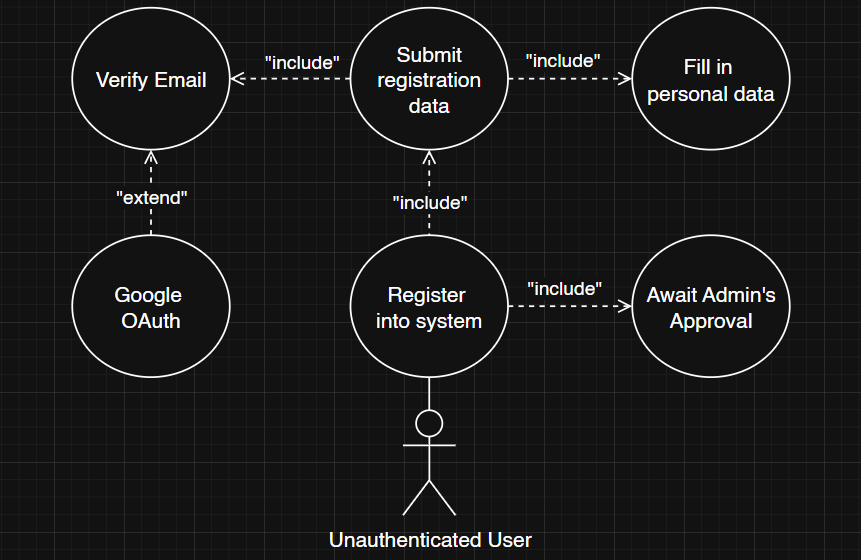
\includegraphics[width=18cm]{"images/umlDiagrams/uml-use-registration.png"}
        \caption{UML Registration Use Case}
        \label{uml-use-registration}
    \end{figure}

    \item \textbf{Document Creation:} The Figure \ref{uml-use-create} represents the process of creating a document within the system by an authenticated user. The actor begins by initiating document creation, which includes multiple dependent steps. The user must upload the document, after which the system checks whether it already exists on the blockchain. The process requires the creator’s approval, the specification of participant IDs, and the subsequent approval of all tagged participants. Once these steps are completed, the creation is confirmed, finalizing the process and preparing the document for secure handling. The diagram emphasizes the structured and multi-party approval workflow that ensures document authenticity and prevents duplication.
    \begin{figure}[H]
        \centering
        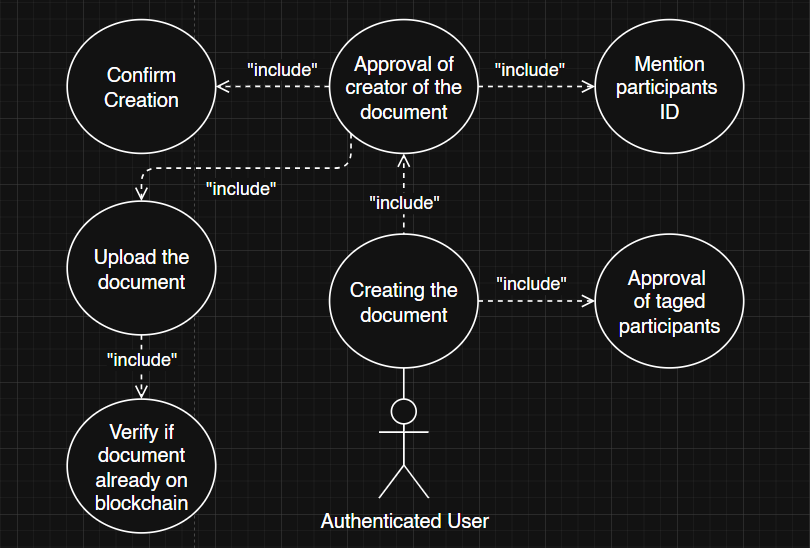
\includegraphics[width=18cm]{"images/umlDiagrams/uml-use-create.png"}
        \caption{UML Document Creation Use Case}
        \label{uml-use-create}
    \end{figure}

    \item \textbf{Document Verification:} The Figure \ref{uml-use-verify} depicts the process of verifying a document by an authenticated user. The actor initiates the verification by uploading the document and providing the participants’ identifiers. The system then calculates the cryptographic hash of the uploaded file and performs a check against existing blockchain records. If a corresponding hash is found, the document is confirmed as authentic and unaltered; otherwise, the system indicates that no match exists. This diagram highlights the structured verification workflow, where hashing and blockchain lookups ensure document integrity and transparency in the verification process.
    \begin{figure}[H]
        \centering
        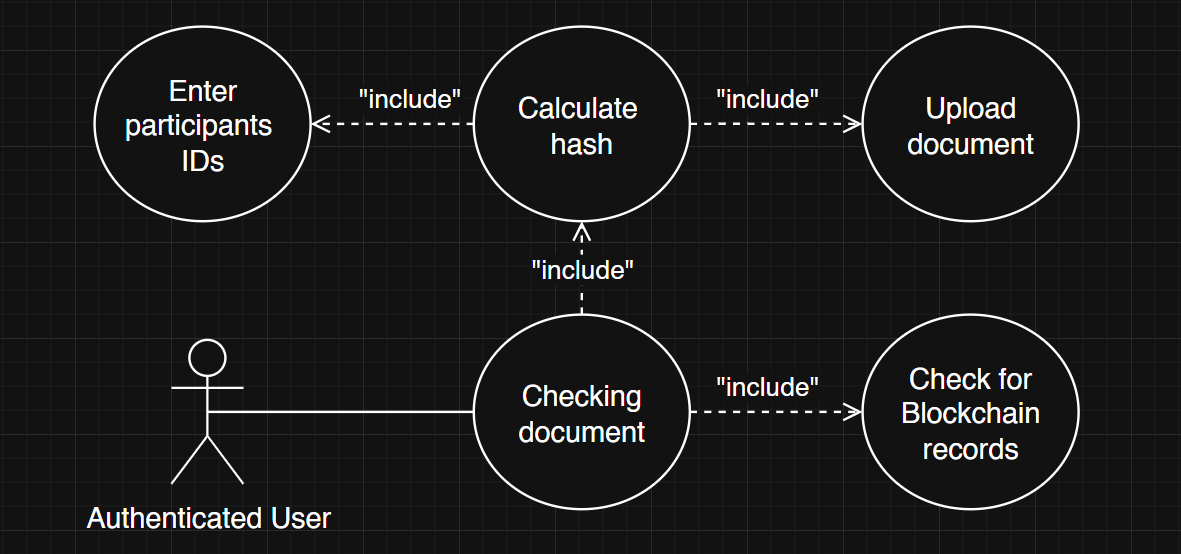
\includegraphics[width=18cm]{"images/umlDiagrams/uml-use-verify.png"}
        \caption{UML Document Verification Use Case}
        \label{uml-use-verify}
    \end{figure}

    \item \textbf{Account Approval:} The Figure \ref{uml-use-approve} models the administrator’s role in approving user registration. The administrator actor is responsible for validating new accounts by checking the uniqueness of the user and comparing the submitted registration data against records provided by the identity provider (IDP). The process also includes requesting personal data through the IDP to confirm authenticity before final approval. This ensures that only legitimate users, whose identities can be verified and who have not previously registered, are granted access to the system. The diagram emphasizes the administrator’s critical role in safeguarding trust, preventing duplicate accounts, and maintaining the integrity of the registration process.
    \begin{figure}[H]
        \centering
        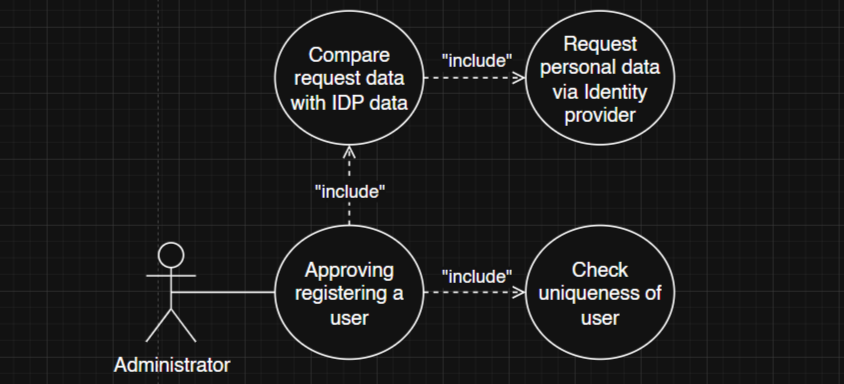
\includegraphics[width=18cm]{"images/umlDiagrams/uml-use-approve.png"}
        \caption{UML Account Approval Use Case}
        \label{uml-use-approve}
    \end{figure}
\end{enumerate}

\subsection{Sequence Diagrams}
The sequence diagrams illustrate the chronological flow of actions and messages for key scenarios, showing how the system components collaborate to achieve the intended operations.\begin{enumerate}
    \item \textbf{Registration process:} The Figure \ref{uml-sequence-registration} illustrates the registration workflow for an unauthenticated user. The process begins when the user initiates registration, which triggers the client interface to start the registration procedure and confirm the initiation with the server. The client then renders the registration window where the user provides personal data. At this point, the server initiates an email verification by sending a code to the user’s email account. The client displays this code input field, and the user submits the verification code to confirm the email. The server validates the code and returns a response, which the client displays as a status message. Once verified, the user submits the full registration data, and the server saves the request, confirms the creation, and the client interface updates the UI to reflect successful registration. This sequence diagram emphasizes the interaction between the user, client UI, server, and email service to ensure secure and validated registration.
    \begin{figure}[H]
        \centering
        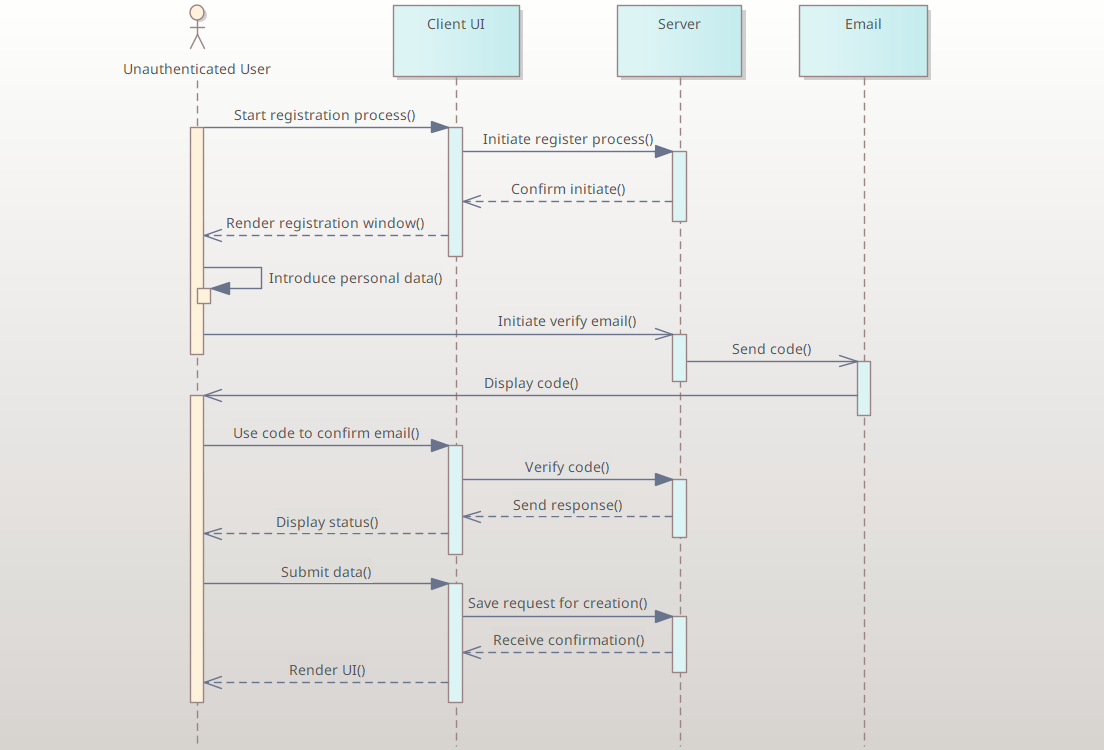
\includegraphics[width=18cm]{"images/umlDiagrams/uml-sequence-registration.png"}
        \caption{UML Registration Sequence}
        \label{uml-sequence-registration}
    \end{figure}

    \item \textbf{Document Creation:} The Figure \ref{uml-use-create} describes the process of document creation by an authorized user. The workflow starts when the user initiates the creation process through the client, which renders the UI. The user uploads the document, provides the participants’ IDs, and confirms the action. The client then sends a request for document creation to the server, which computes the hash of the file and checks the blockchain for existing records. If no duplicate is found, the server proceeds by distributing the document to all listed participants for approval. Once the approvals are collected, the server creates a new immutable record on the blockchain and confirms its creation. At the same time, a reference to the new document is stored in the database, linking it to the user’s account. Finally, the confirmation is returned to the client, which updates the user interface with the new document’s details. This sequence diagram highlights the coordinated interaction between client, server, blockchain, and database to ensure document integrity, approval, and traceability.
    \begin{figure}[H]
        \centering
        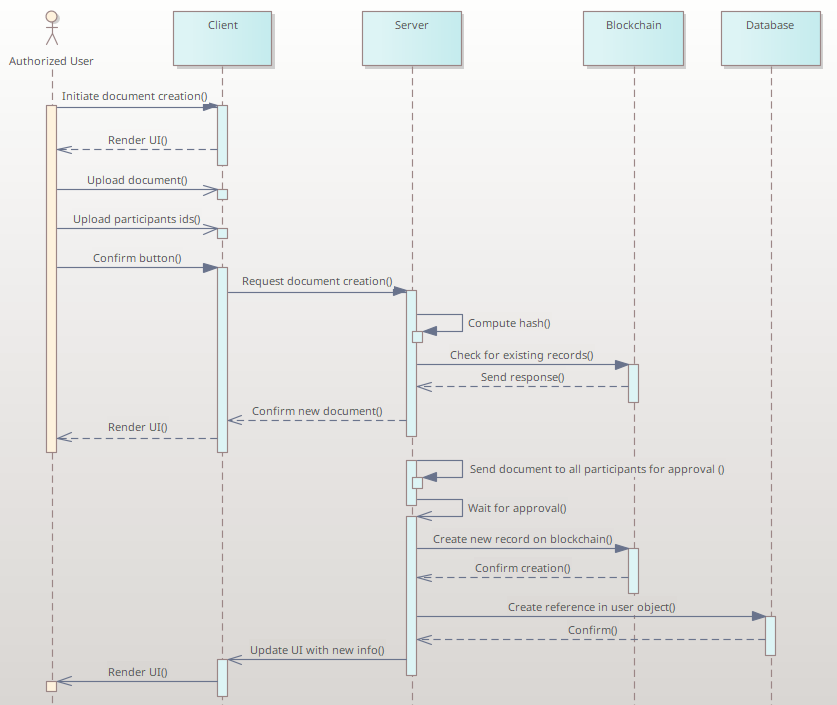
\includegraphics[width=18cm]{"images/umlDiagrams/uml-sequence-create.png"}
        \caption{UML Document Creation Sequence}
        \label{uml-sequence-create}
    \end{figure}

    \item \textbf{Document Verification:} The Figure \ref{uml-sequence-verify} shows the workflow for document verification by an authorized user. The process begins when the user initiates the verification through the client interface, which renders the UI. The user uploads the document and enters the participants’ IDs before confirming the action. The client then sends a verification request to the server. The server computes a cryptographic hash of the uploaded file and queries the blockchain to check whether a matching record already exists. The blockchain responds with the result of the lookup, which the server forwards back to the client. Finally, the client displays the verification outcome to the user. This diagram highlights the critical interaction between user actions, system components, and blockchain infrastructure to ensure document authenticity and integrity.
    \begin{figure}[H]
        \centering
        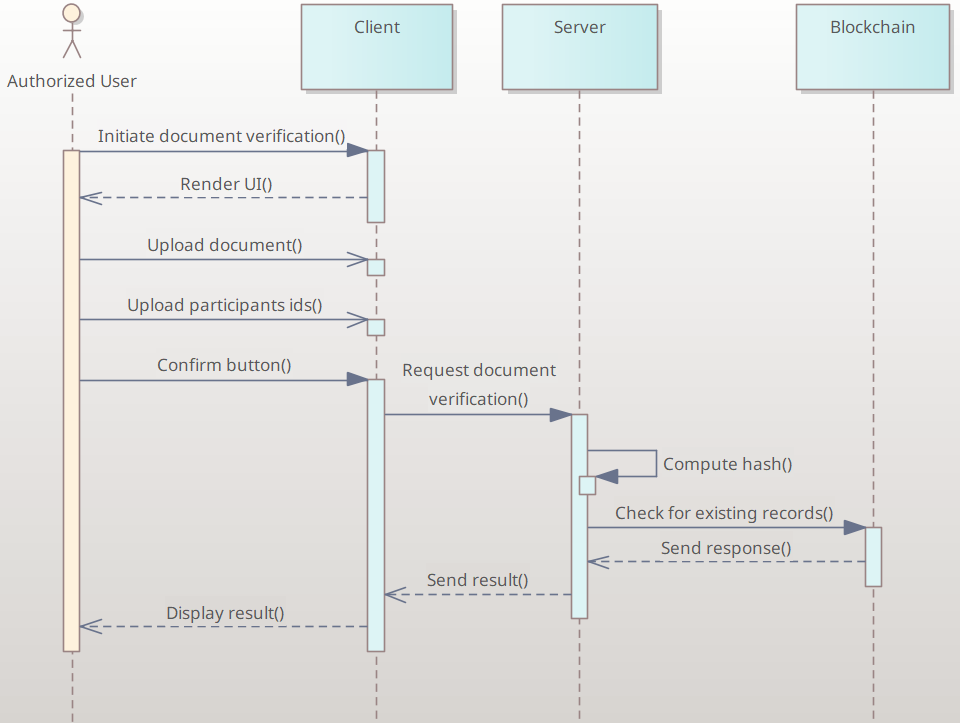
\includegraphics[width=18cm]{"images/umlDiagrams/uml-sequence-verify.png"}
        \caption{UML Document Verification Sequence}
        \label{uml-sequence-verify}
    \end{figure}

    \item \textbf{Account Approval:} The Figure \ref{uml-sequence-approve} illustrates the user account approval process managed by the administrator. The flow begins when the administrator requests pending registration data for review, which the server provides to the admin panel. To validate the registration, the server queries the Identity Provider (IDP) for personal data associated with the submitted IDNP and returns the response. The administrator then compares the provided information against the IDP data. If the data is valid, the administrator approves the account creation. The server processes this approval by generating a new user object in the database, after which a confirmation of account creation is returned to the administrator. This diagram highlights the administrator’s critical role in ensuring user identity verification and the coordinated interaction between the server, identity provider, and database during registration approval.
    \begin{figure}[H]
        \centering
        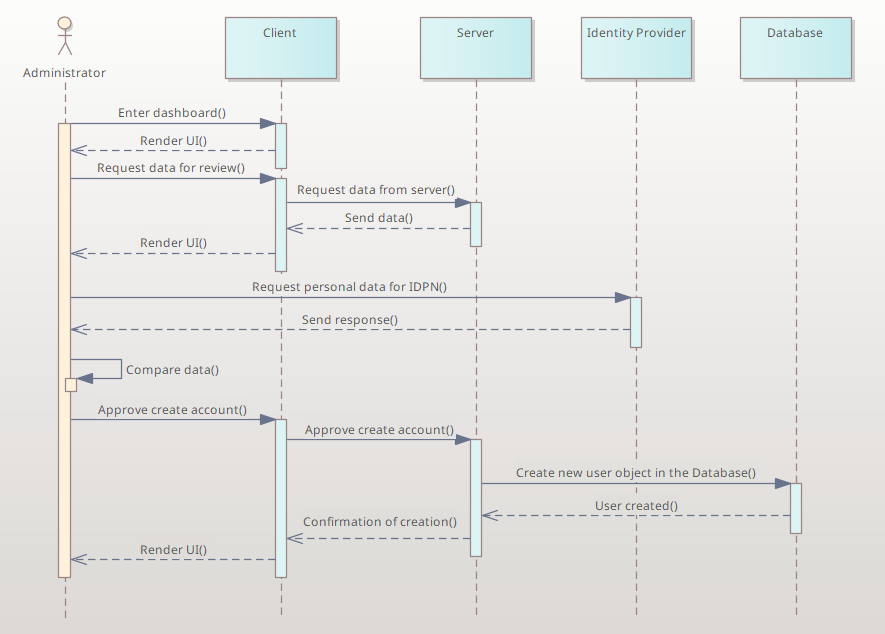
\includegraphics[width=18cm]{"images/umlDiagrams/uml-sequence-approve.png"}
        \caption{UML Account Approval Sequence}
        \label{uml-sequence-approve}
    \end{figure}
\end{enumerate}


\section{Structural Modeling}
This section presents the structural view of the system, focusing on the static aspects of its architecture. Structural modeling helps define the main components, their responsibilities, and the relationships between them.

\subsection{Class Diagram}
The Figure \ref{uml-class-core-domain} models the core entities and relationships within the document notarization system. At the center is the User class, which contains attributes such as ID, full name, email, phone, status, role, and timestamps, alongside methods for document creation, signing, declining, and verification. Each user is assigned a Role, which defines permissions and enforces access control.

The Document class represents notarized files with properties like ID, title, owner, status, storage reference, size, and creation details. Its methods manage the signing workflow, including adding participants, submitting for signing, and finalizing signatures. A document is linked to multiple Participants, each of whom has a role, status, and the ability to either sign or decline. These actions generate corresponding Signatures, which record details such as participant ID, signature type, reference, and timestamp.

\begin{figure}[H]
    \centering
    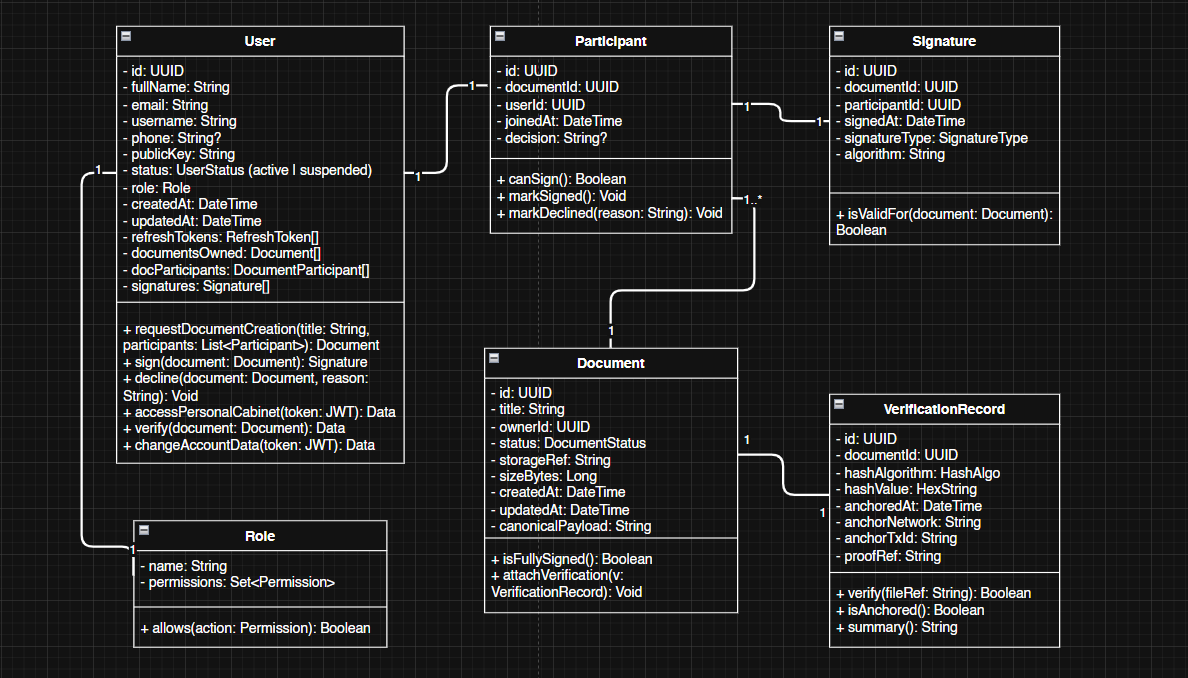
\includegraphics[width=18cm]{"images/umlDiagrams/uml-class-core-domain.png"}
    \caption{UML Core Domain Class Model}
    \label{uml-class-core-domain}
\end{figure}

Additionally, the system maintains VerificationRecords, which store blockchain-related data like hash values, algorithms, anchoring timestamps, and network references. These records provide functions to verify integrity, check anchoring, and generate summaries.

Altogether, this diagram highlights how users, roles, documents, participants, signatures, and verification records interact. It reflects a cohesive domain model where documents are securely managed, signed by multiple parties, and validated against blockchain anchors to ensure integrity and trustworthiness.

\newpage
\section{Figma User Interface Mockups}

The landing page (Figure \ref{landing1}) is the first page seen by the user when entering the site, so it gives the user a clear description of the functionality the service provides.

\begin{figure}[H]
    \centering
    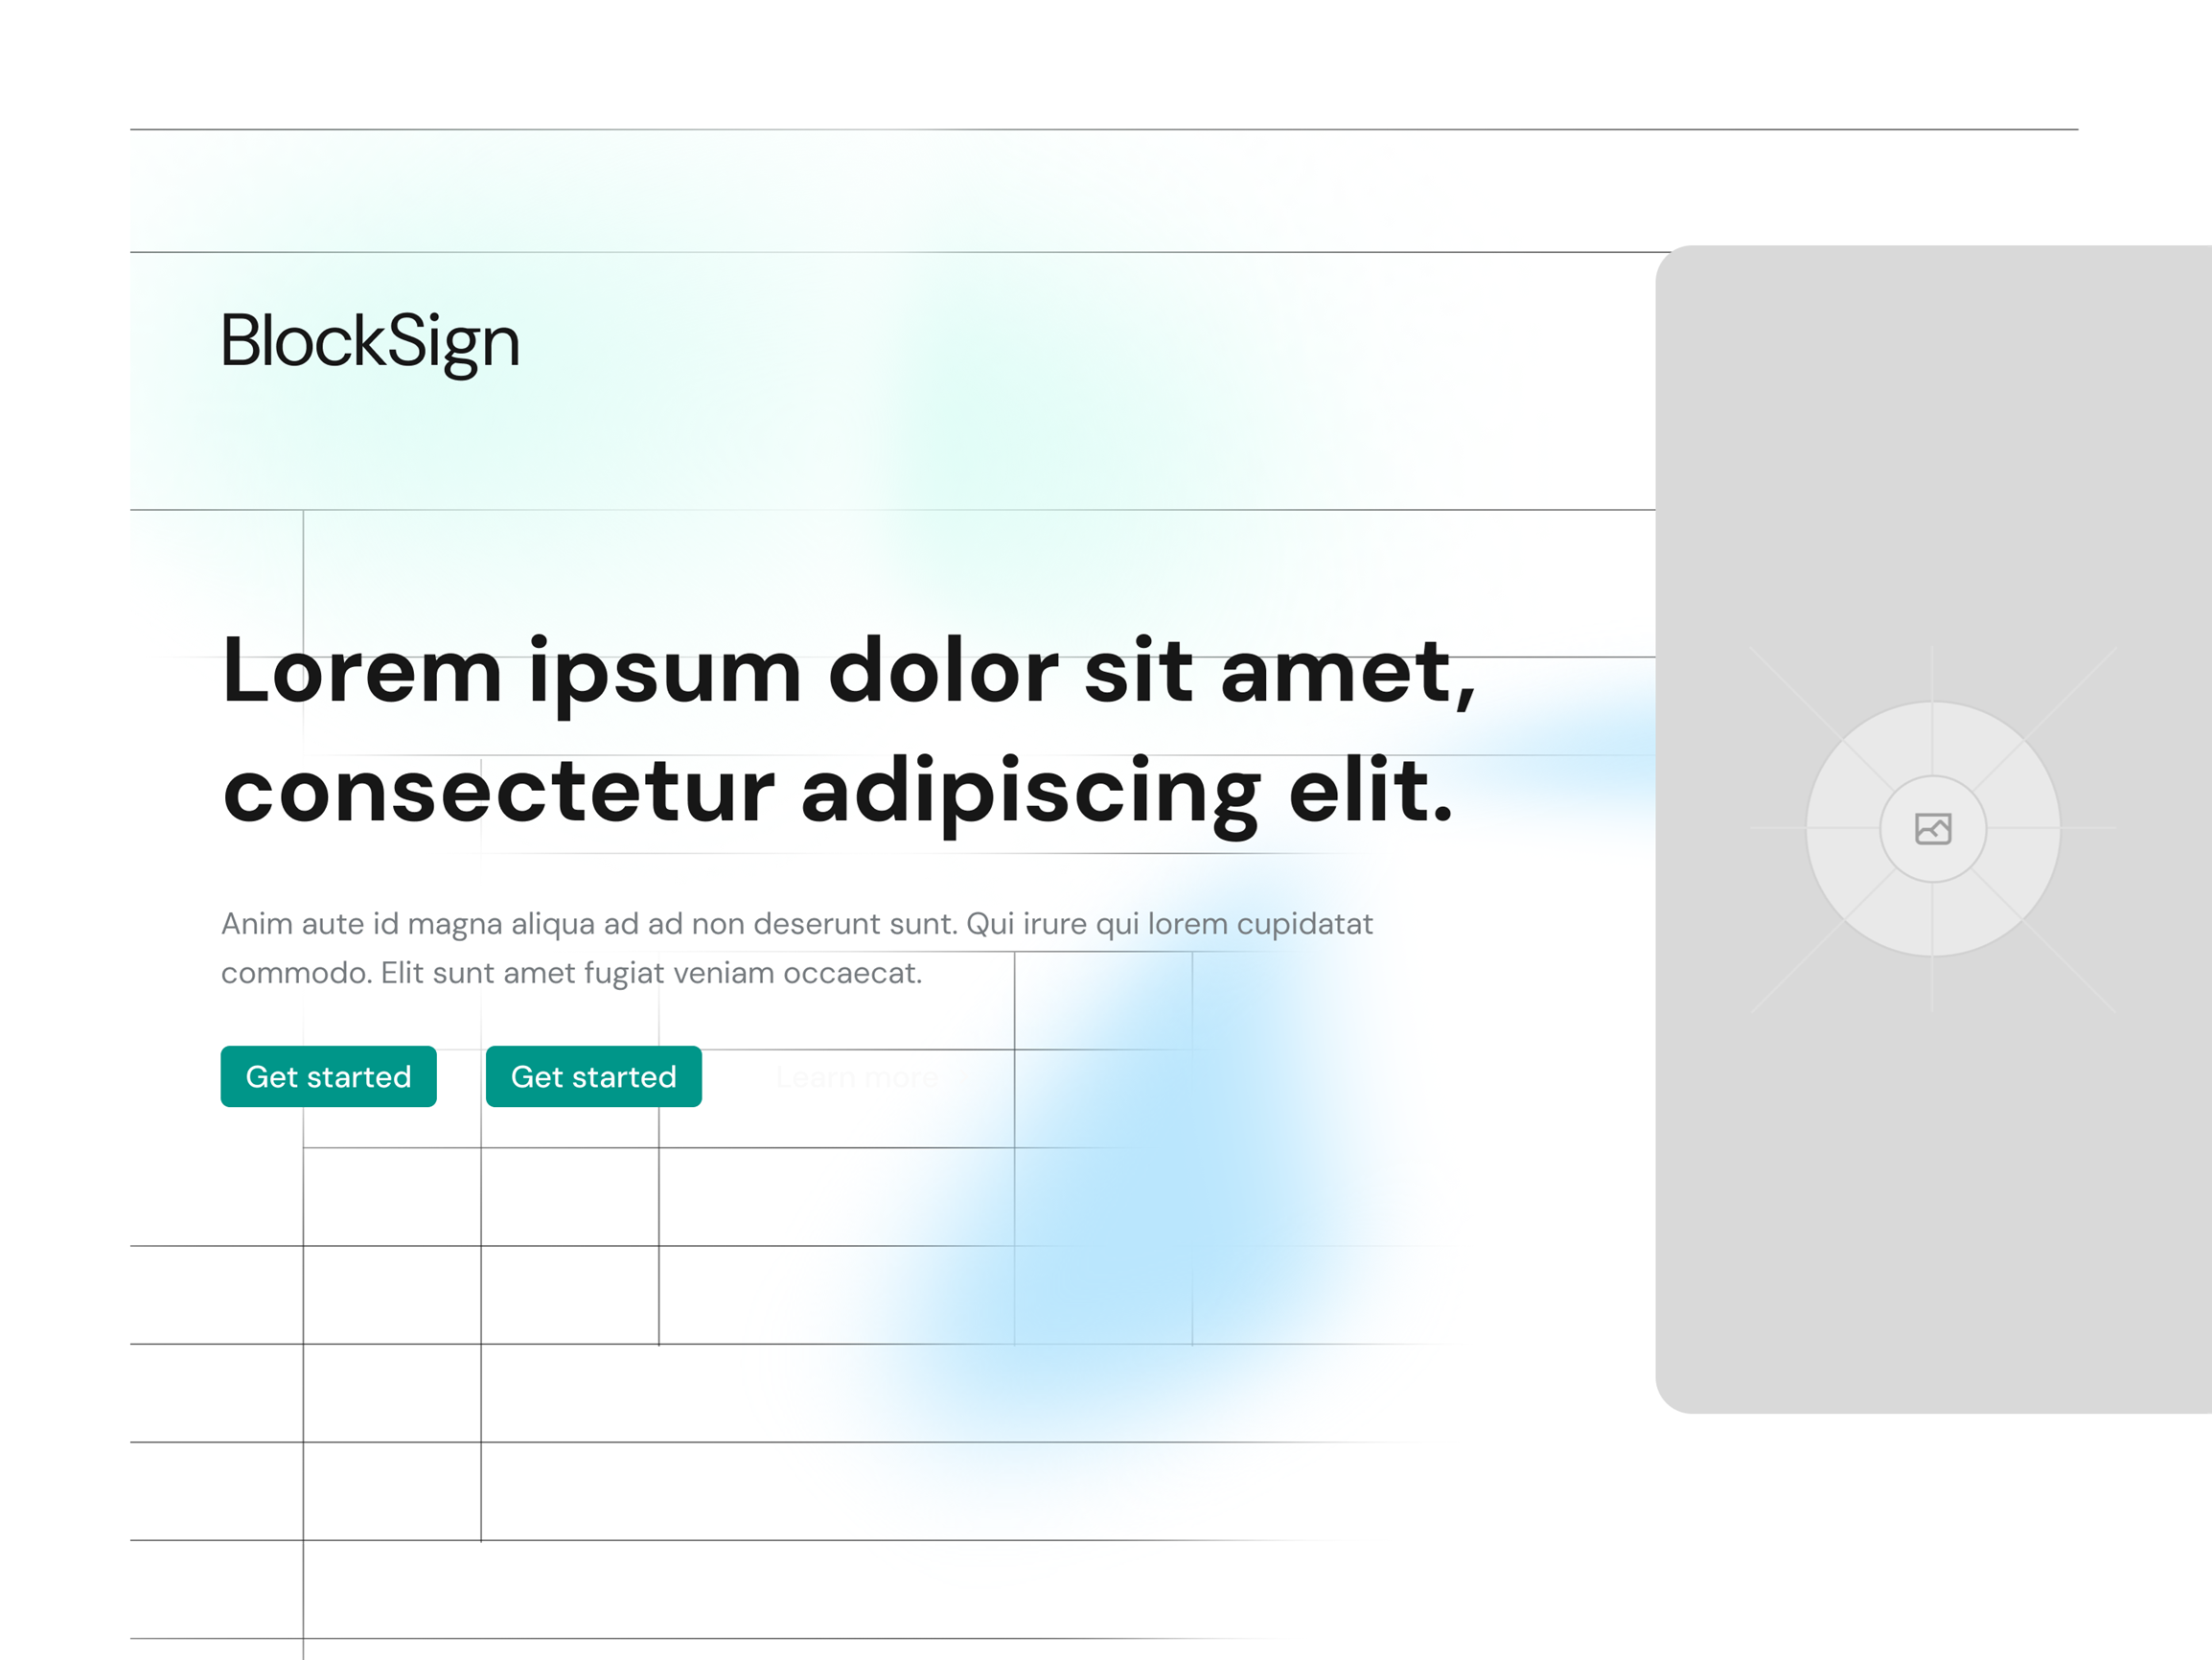
\includegraphics[width=18cm, height=20cm, keepaspectratio]{"images/figmaUI/landing-top.png"}
    \caption{Landing page}
    \label{landing1}
\end{figure}

\newpage
The login page (Figure \ref{login}) has the possibility of entering via email and password, as well as entering through existing accounts in services such as Google. 


\begin{figure}[H]
    \centering
    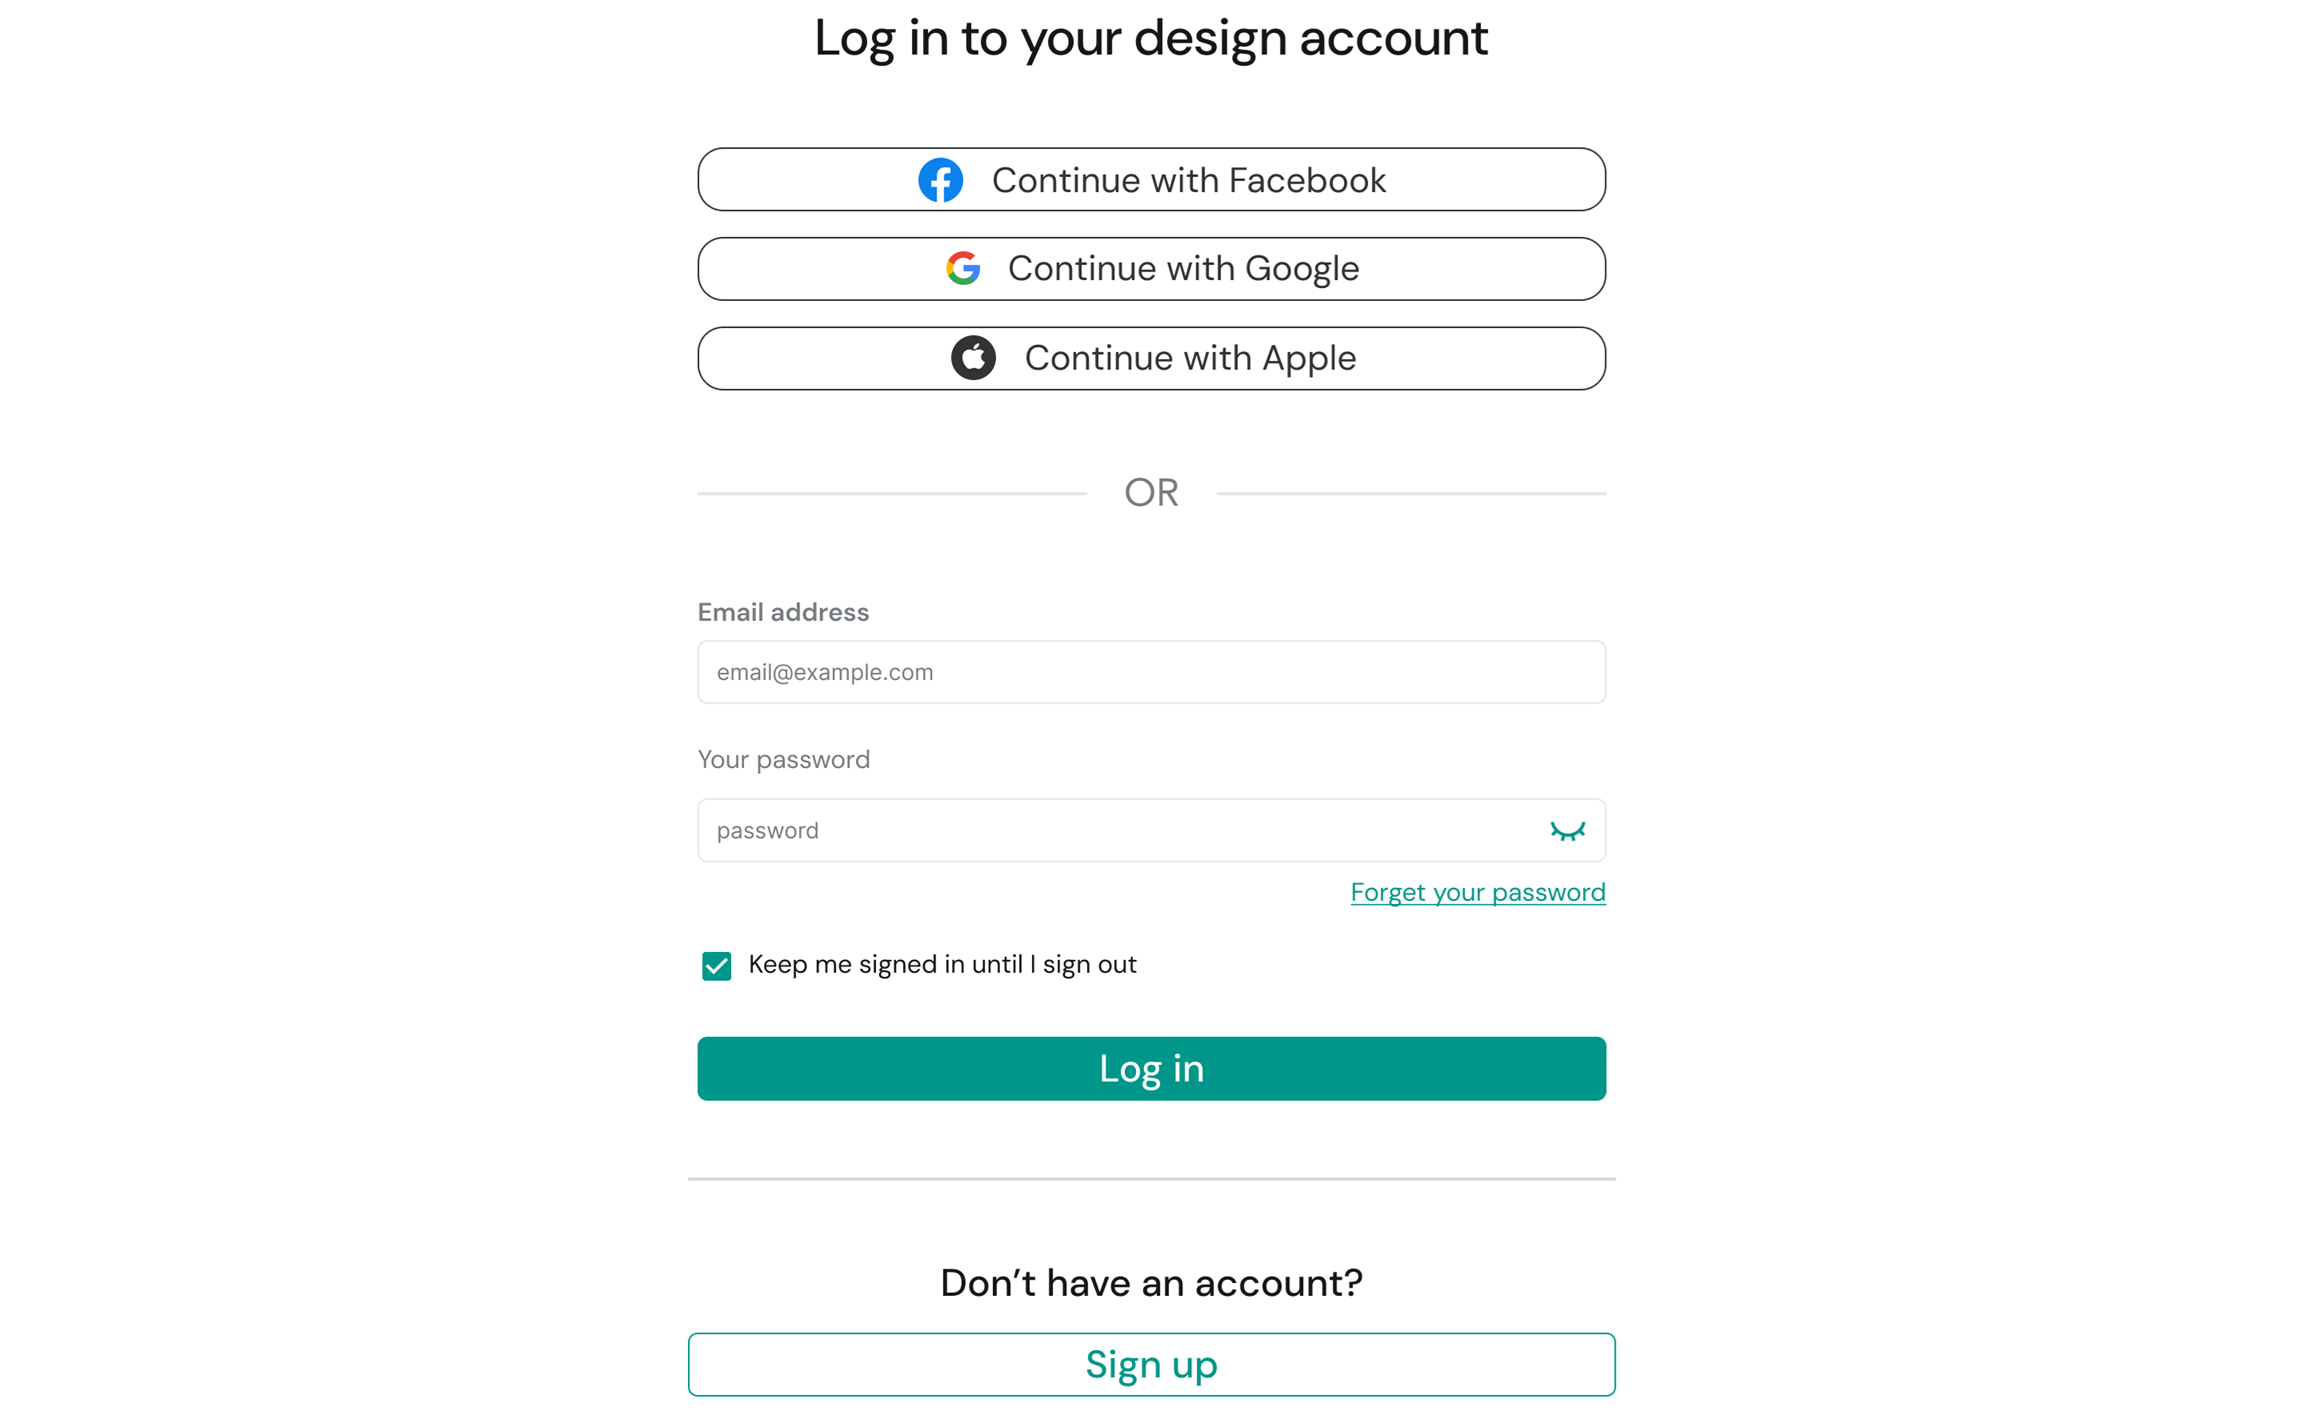
\includegraphics[width=18cm]{"images/figmaUI/login-crop.png"}
    \caption{Login page}
    \label{login}
\end{figure}

\newpage
The registration page (Figure \ref{register}) provides the user with the possibility to create an account in the service and lets the use of other services such as Google to provide the information needed to service. 


\begin{figure}[H]
    \centering
    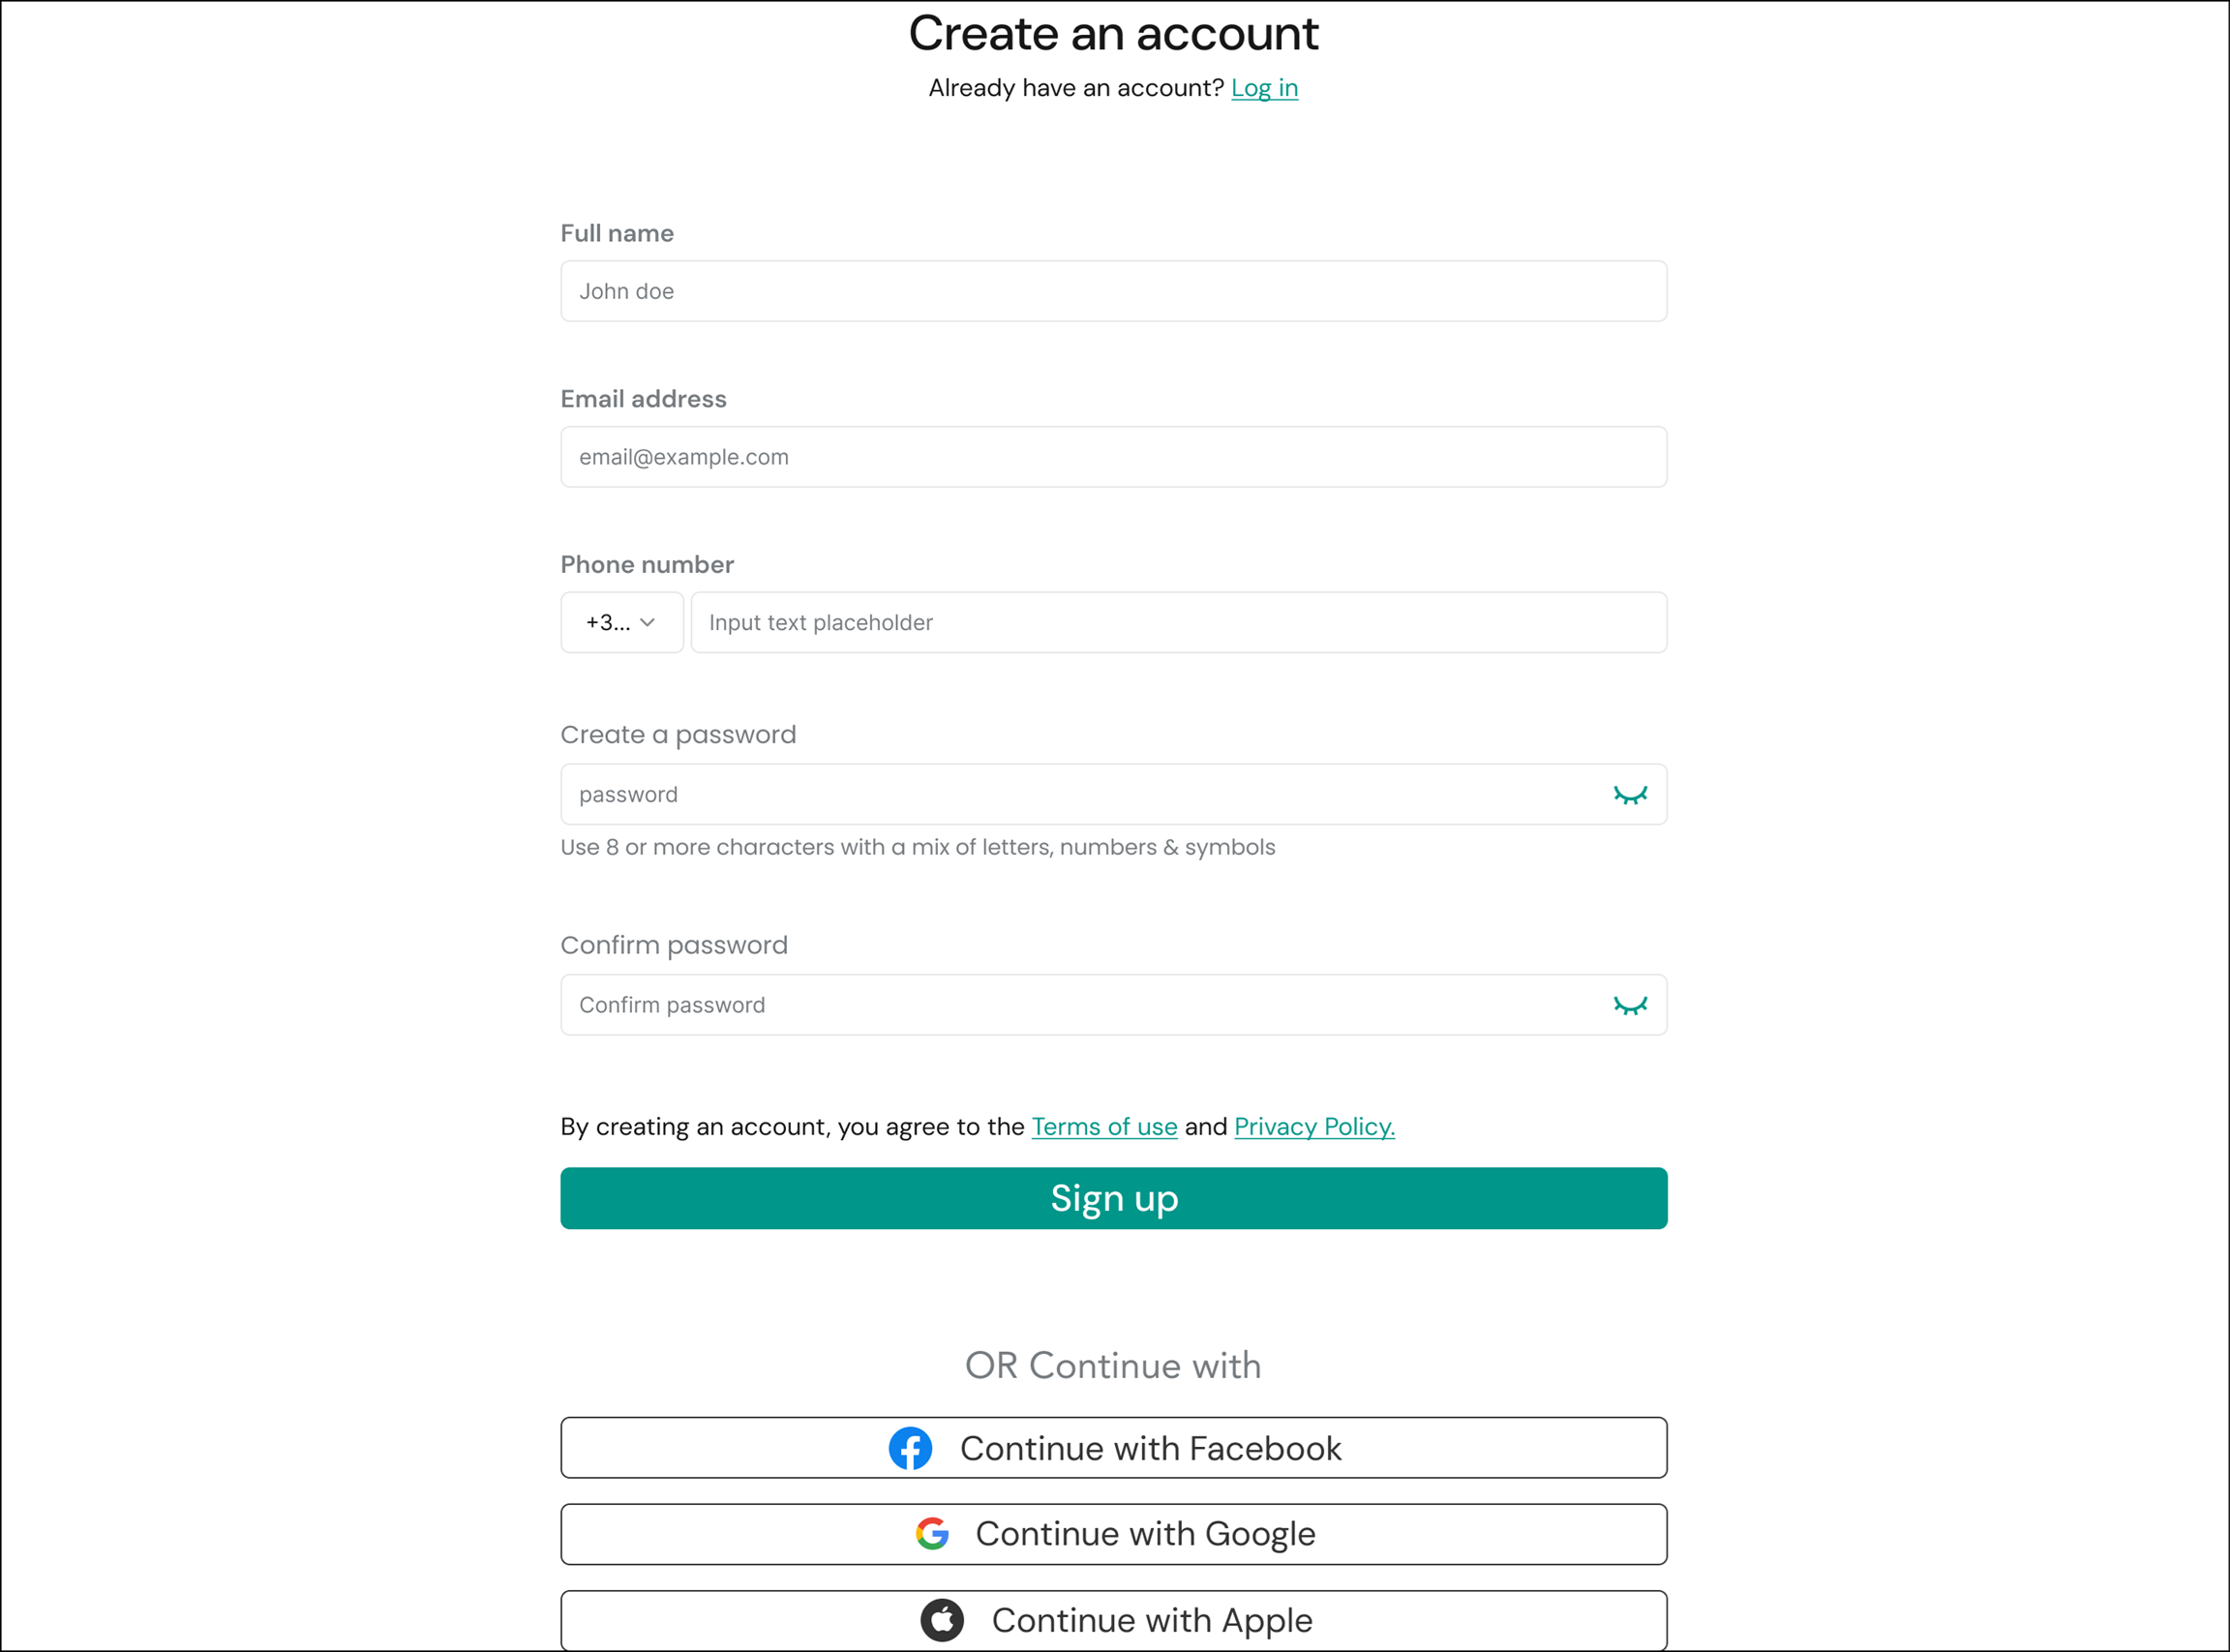
\includegraphics[width=18cm]{"images/figmaUI/register1-crop.png"}
    \caption{Register page - User info}
    \label{register}
\end{figure}

\newpage
The second step of registration (Figure \ref{registerstep2}) is a confirmation of the user's email. 


\begin{figure}[H]
    \centering
    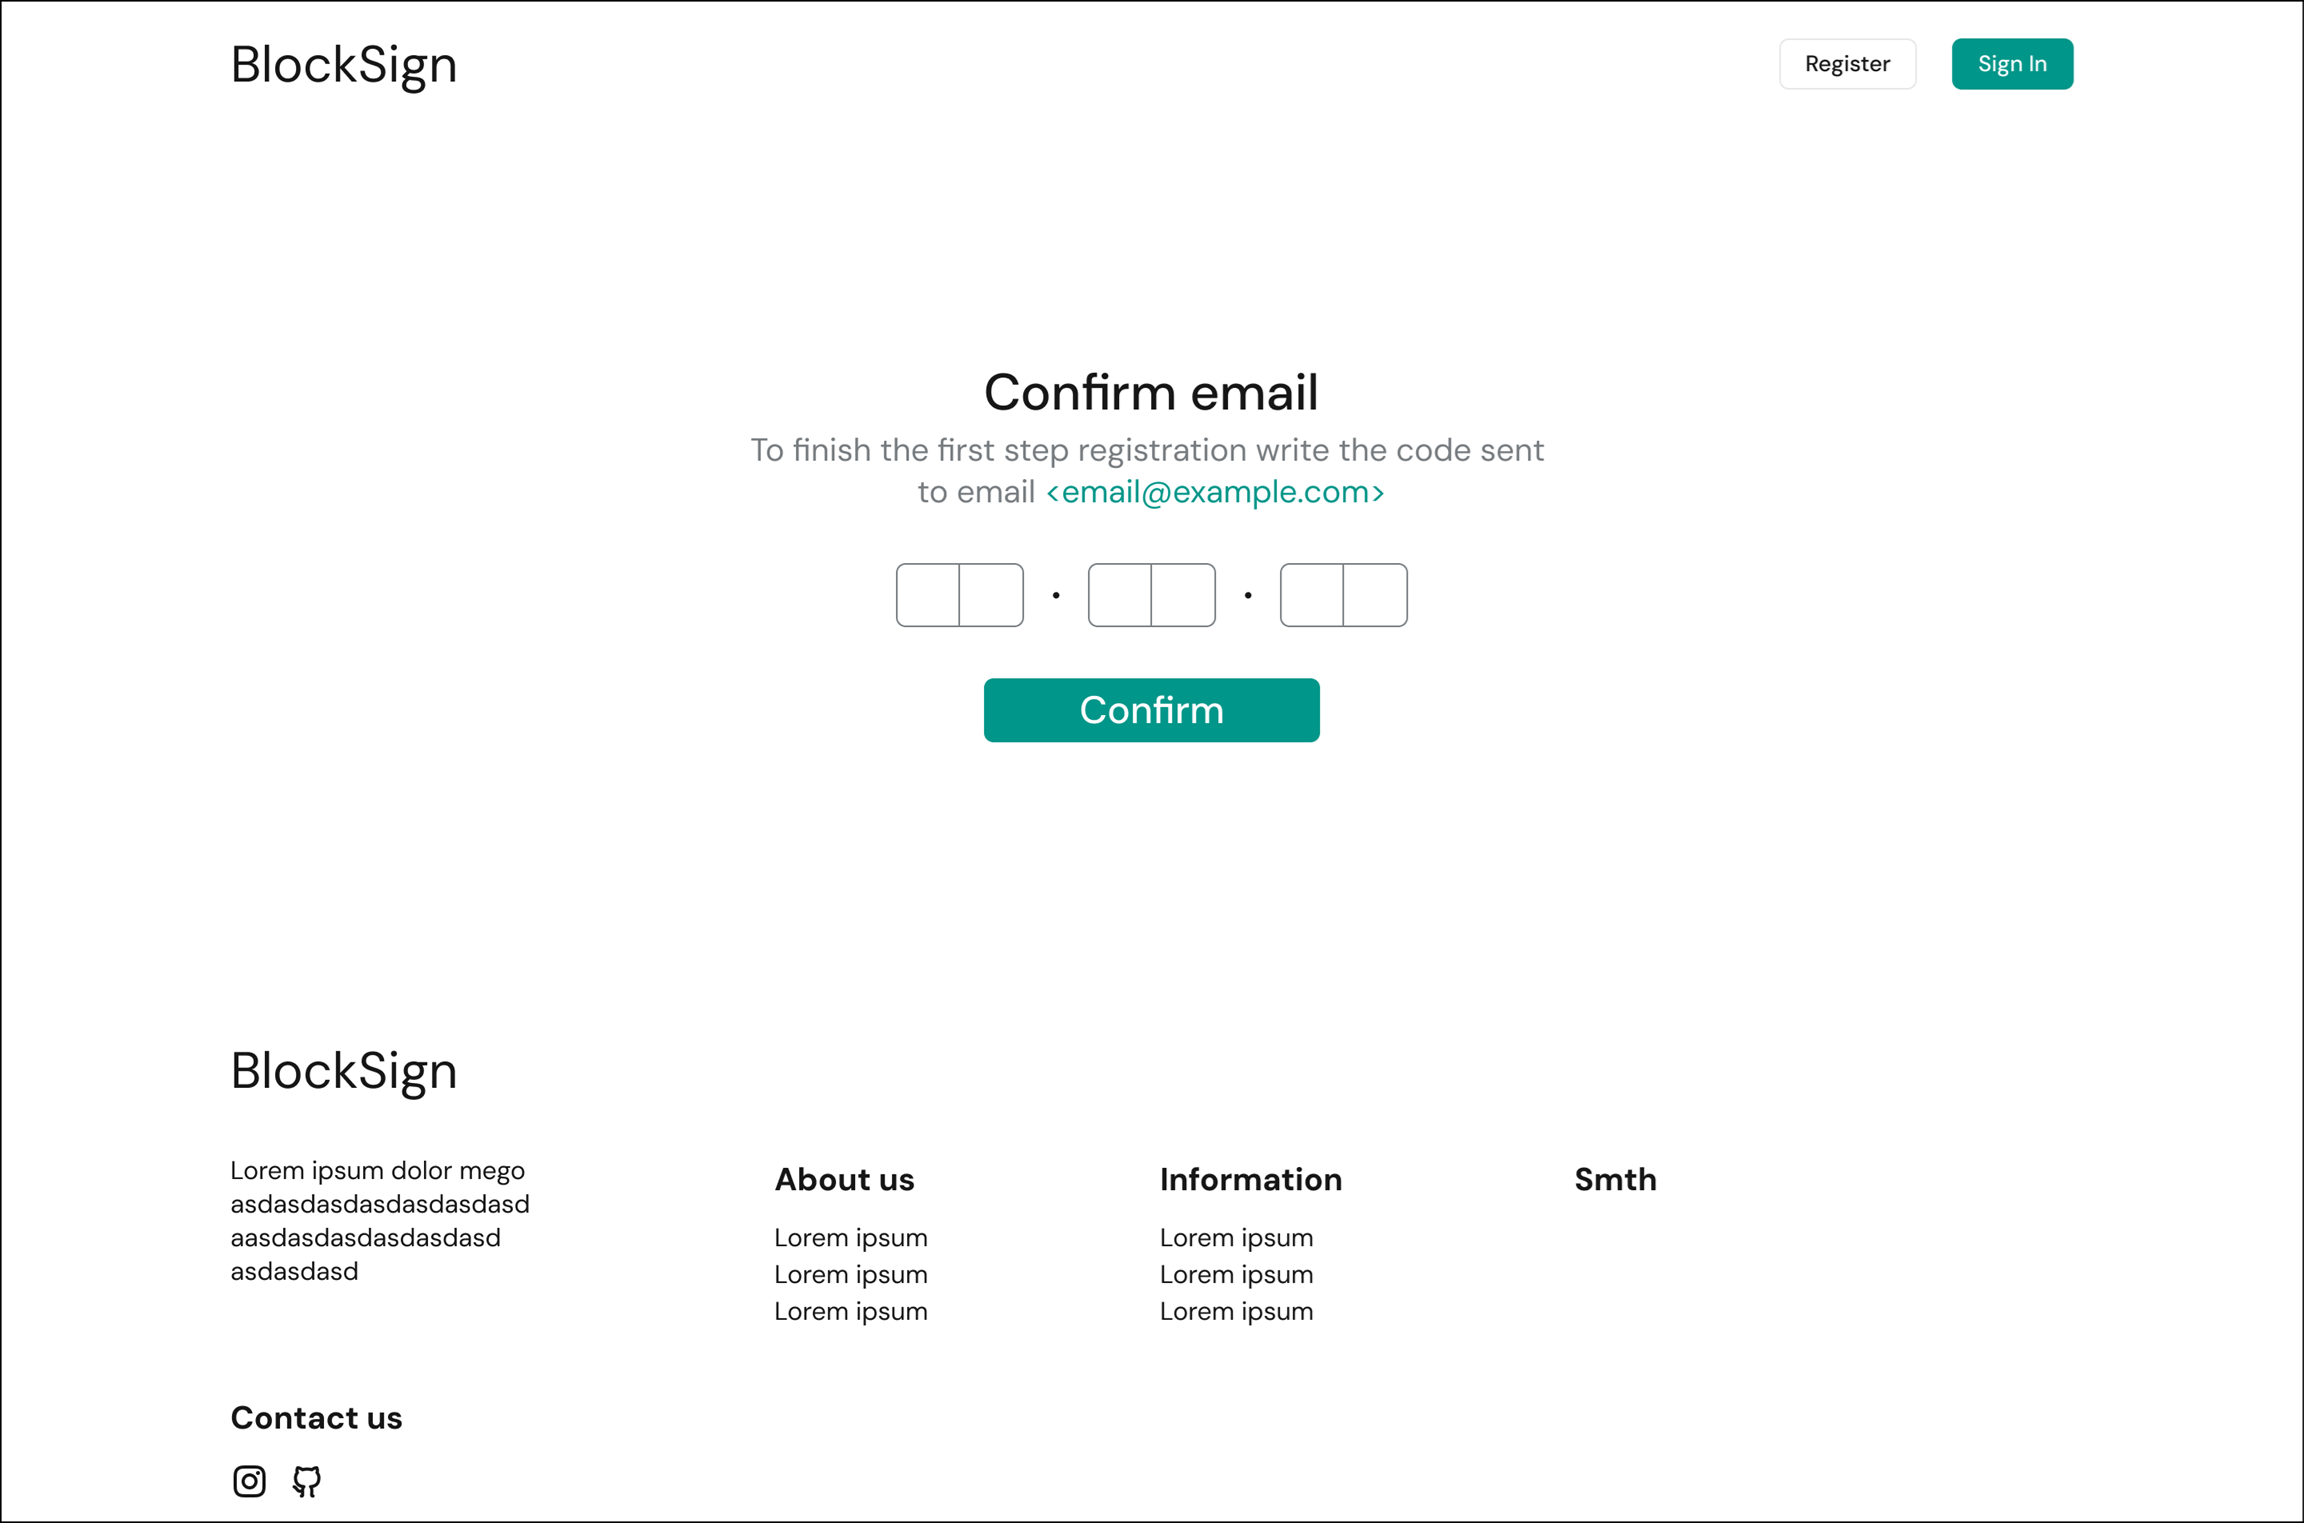
\includegraphics[width=18cm]{"images/figmaUI/registerstep2.png"}
    \caption{Register - Verifying the email}
    \label{registerstep2}
\end{figure}


The third step of registration (Figure \ref{registerstep3}) is a confirmation of identity using sensitive personal data that is not stored or used after verification.


\begin{figure}[H]
    \centering
    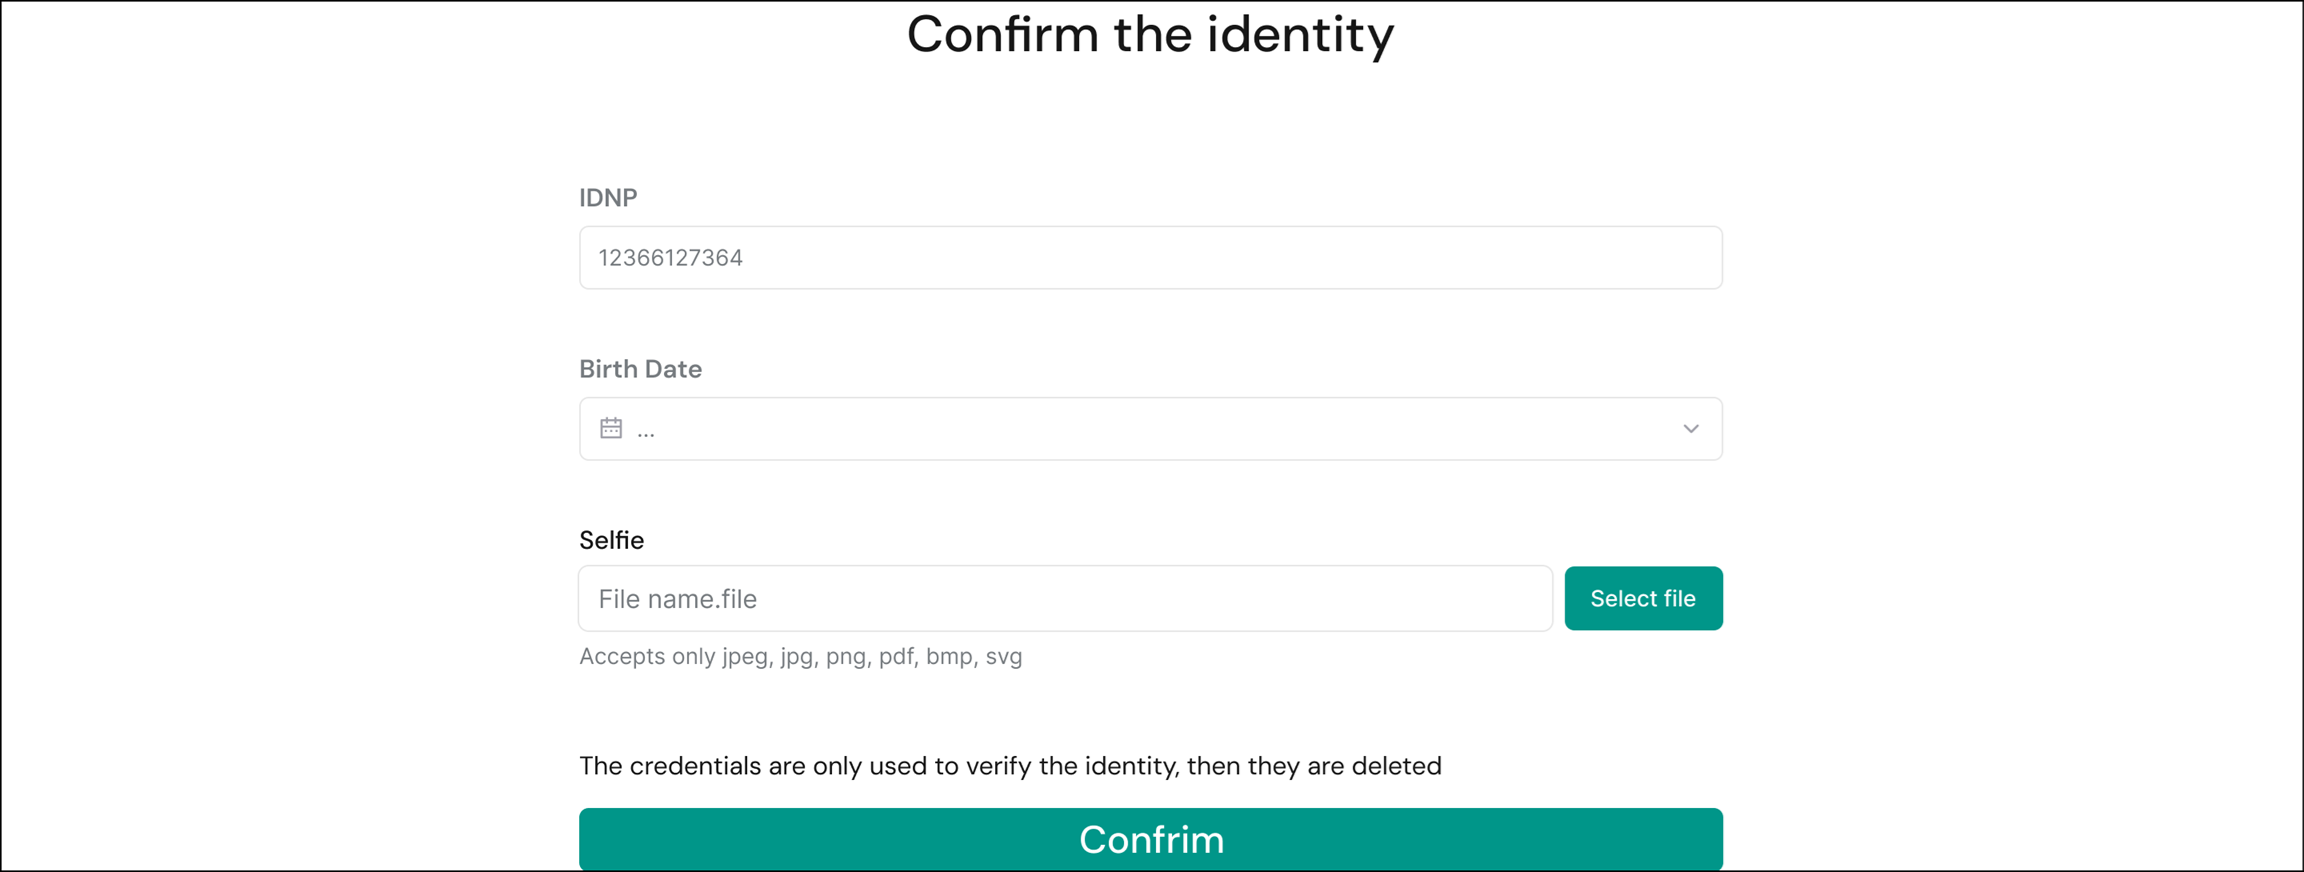
\includegraphics[width=18cm]{"images/figmaUI/register3-crop.png"}
    \caption{Register - Confirming the identity}
    \label{registerstep3}
\end{figure}

\newpage
Then the user sees the successful finish (Figure \ref{documentspage1}) screen and is redirected to his account.


\begin{figure}[H]
    \centering
    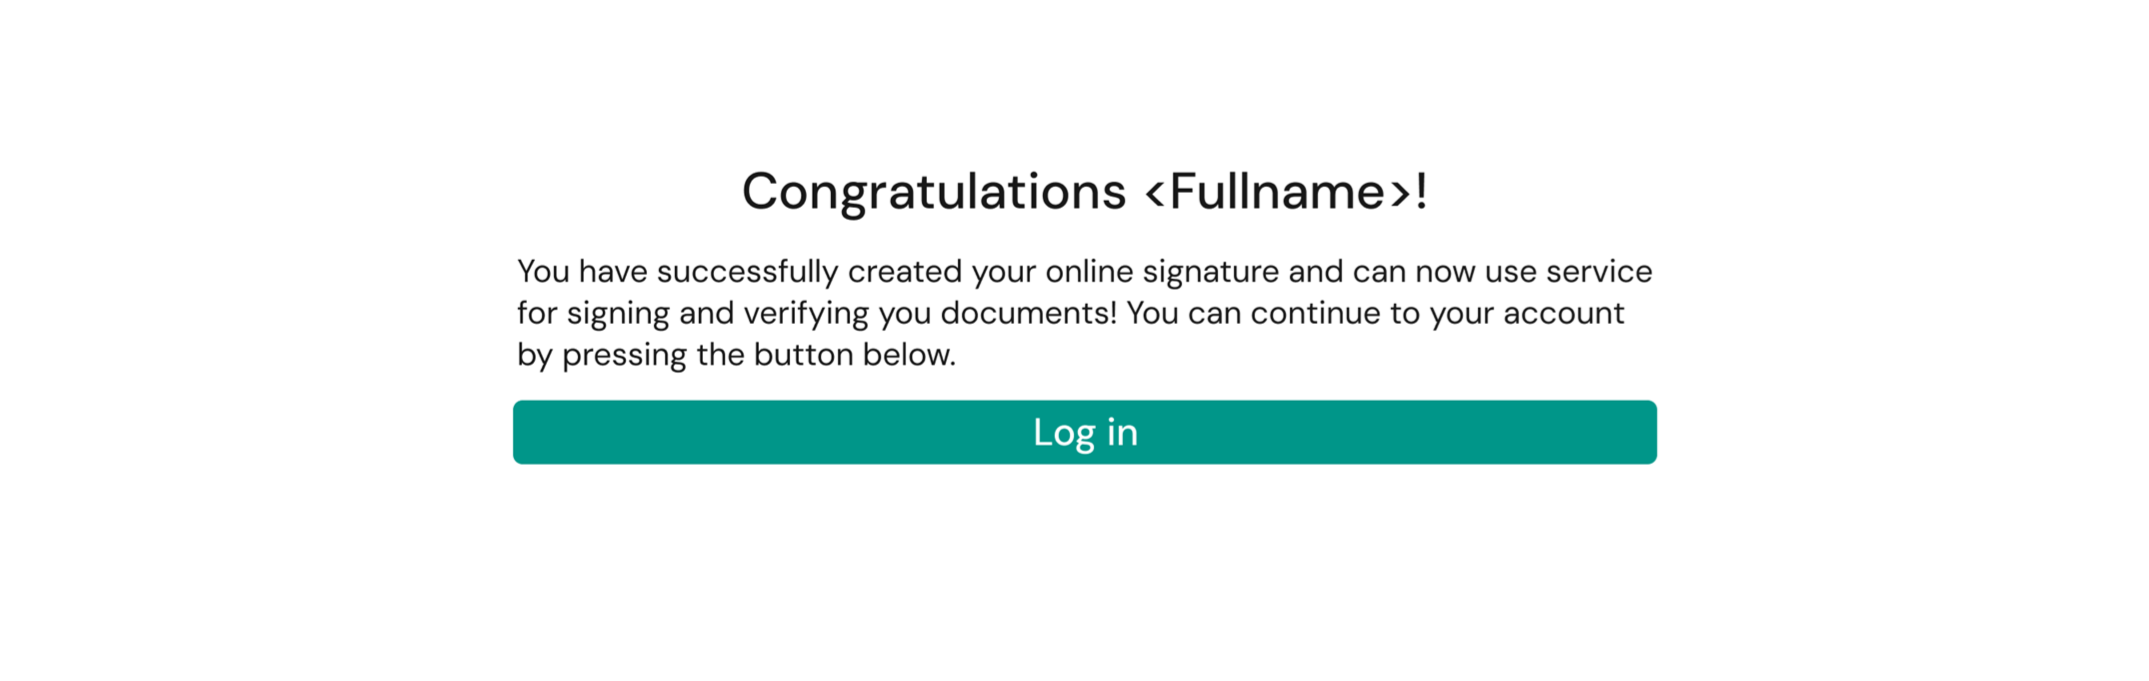
\includegraphics[width=18cm]{"images/figmaUI/successregister.png"}
    \caption{Register - Successful finish}
    \label{successregister}
\end{figure}

\newpage
When authorized user gets access to the pages: documents( Figures \ref{documentspage1}, \ref{documentspage2}), account (Figures \ref{accountspage-account}, \ref{accountspage-protection}, \ref{accountspage-documents} )


The documents page has 2 main functionalities - uploading (Figure \ref{documentspage1}) and creating a session of signing the document, and second - verifying (Figure \ref{documentspage2}) if the file with the given users was ever signed. 


\begin{figure}[H]
    \centering
    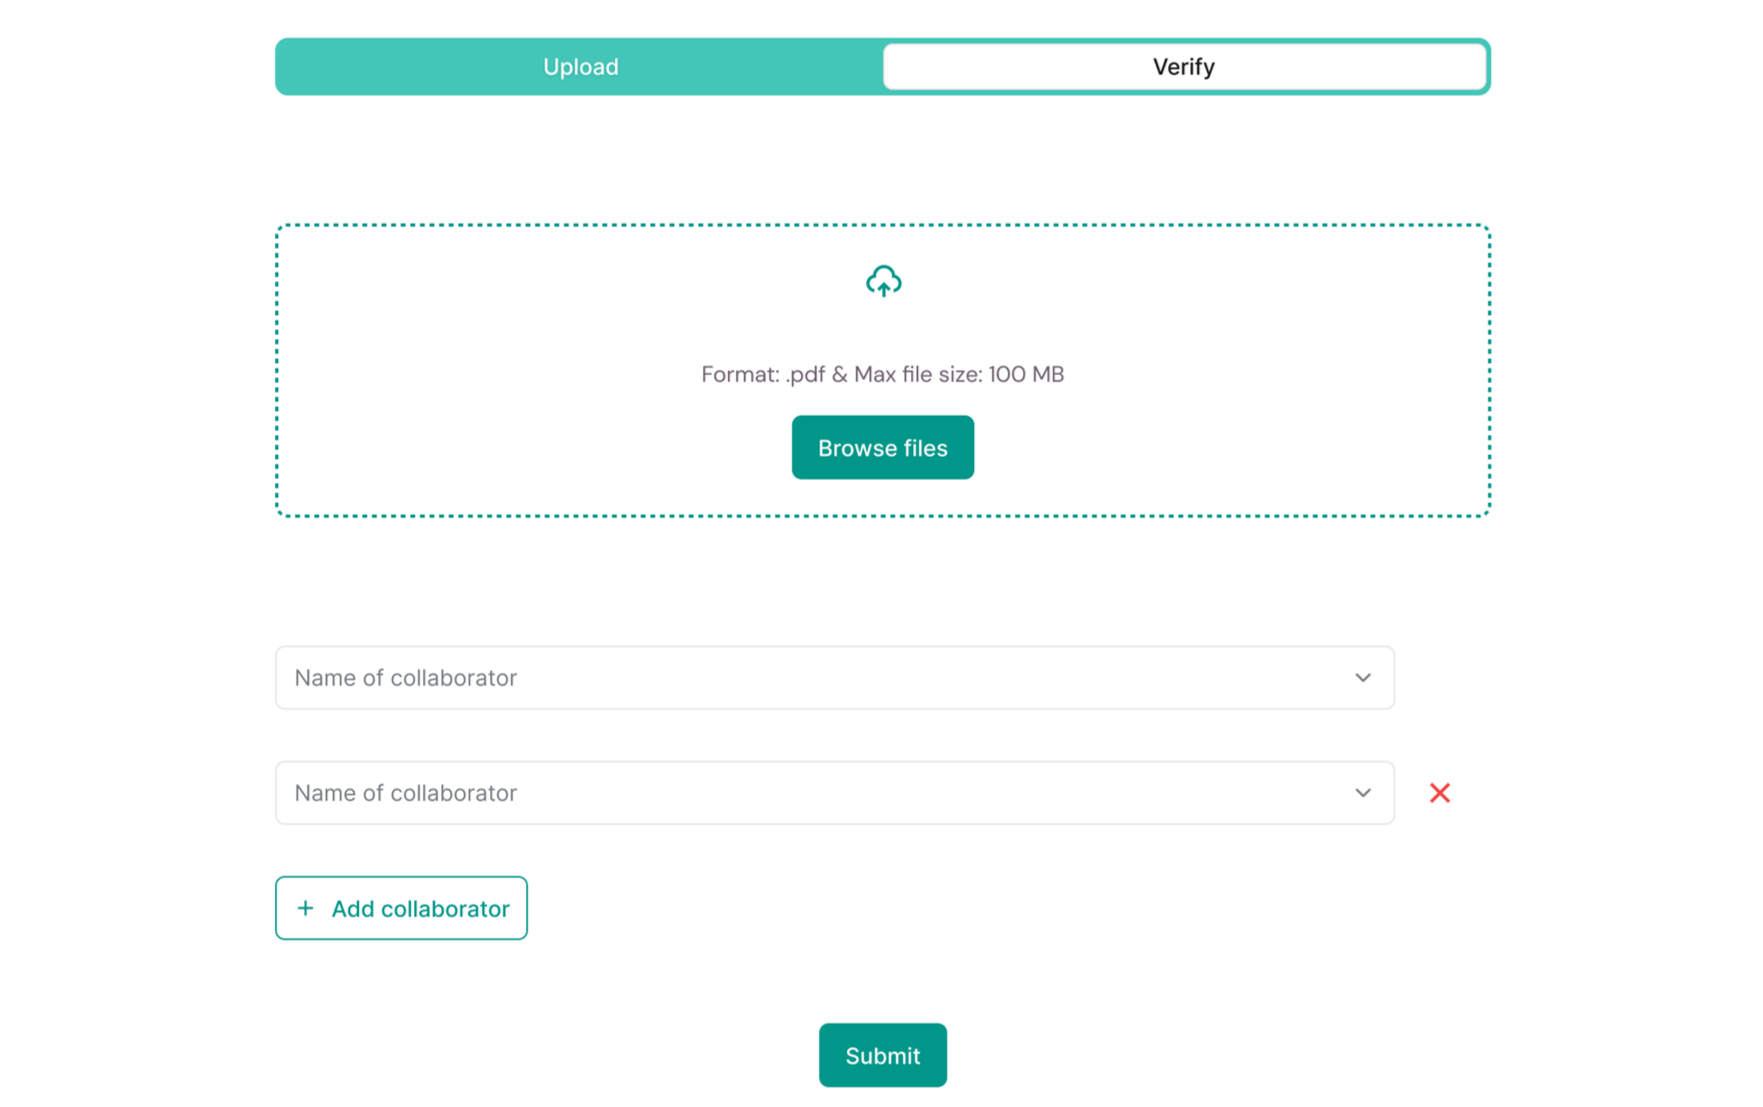
\includegraphics[width=18cm]{"images/figmaUI/documentspage1-crop.png"}
    \caption{Documents page - Verify an existing document}
    \label{documentspage1}
\end{figure}


The results of verifying might be only exists (Figure \ref{documents-exists}) or does not exist (Figure \ref{documents-noinstance}).


\begin{figure}[H]
    \centering
    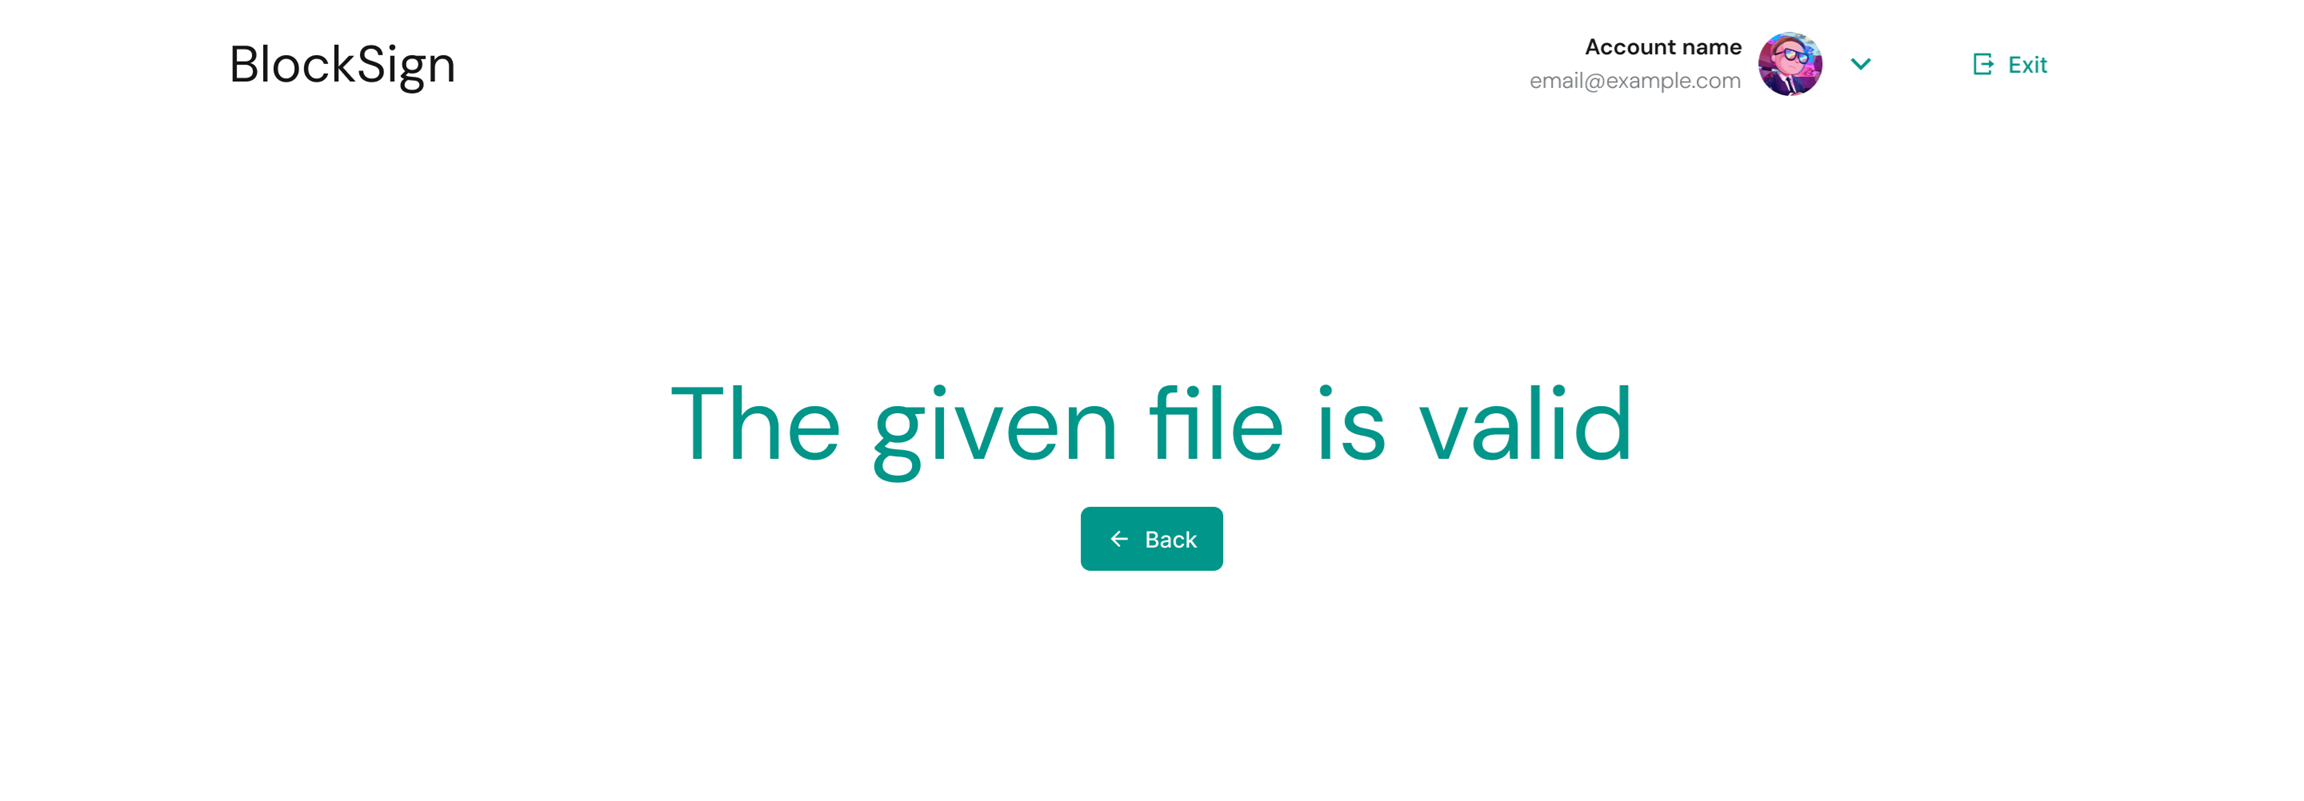
\includegraphics[width=18cm]{"images/figmaUI/success-crop.png"}
    \caption{Documents page - Existing instance of document}
    \label{documents-exists}
\end{figure}


\begin{figure}[H]
    \centering
    
\includegraphics[width=18cm]{"images/figmaUI/unsuccess-crop.png"}
    \caption{Documents page - Not existing instance of document}
    \label{documents-noinstance}
\end{figure}


On the upload option (Figure \ref{documentspage2}) the session of the signing the document is created by adding the sides of the signing via account name/id. 


\begin{figure}[H]
    \centering
    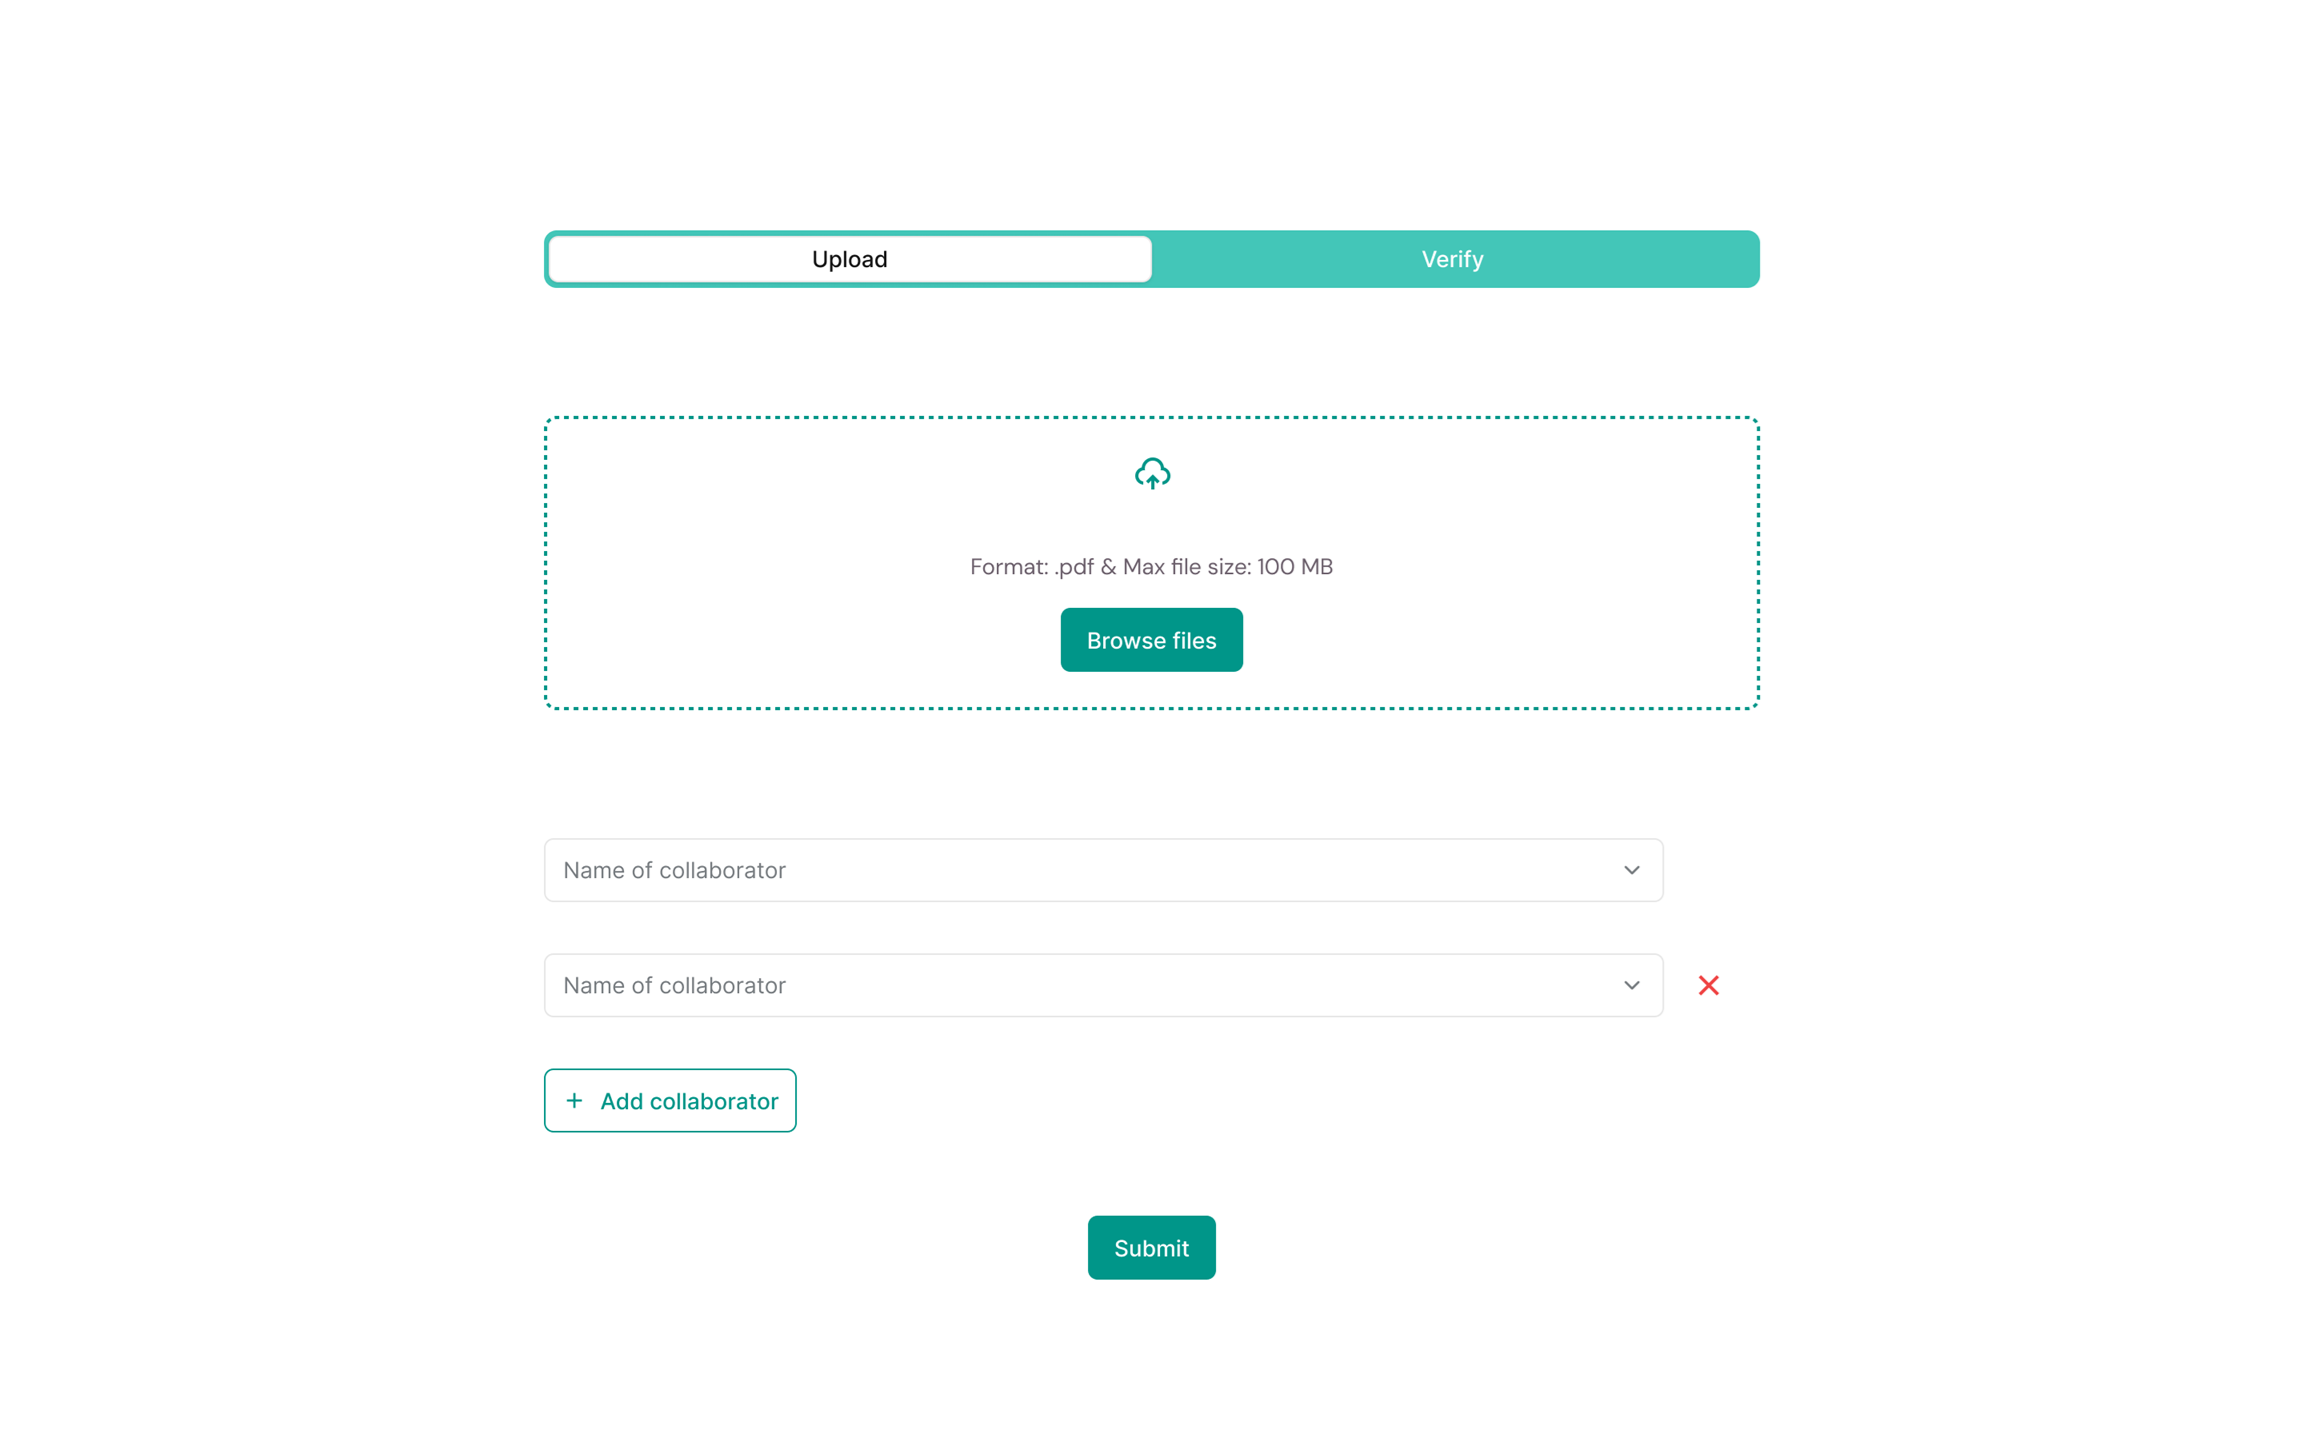
\includegraphics[width=18cm]{"images/figmaUI/documentspage2-crop.png"}
    \caption{Documents page - Upload and sign the document}
    \label{documentspage2}
\end{figure}

\newpage
The account page gives the ability to manipulate the user account(Figure \ref{accountspage-account}) and protection(Figure \ref{accountspage-protection}) as well as view and sign the documents(Figure \ref{accountspage-documents}).

The account tab (Figure \ref{accountspage-account}) has the customization of the previously introduced info.

\begin{figure}[H]
    \centering
    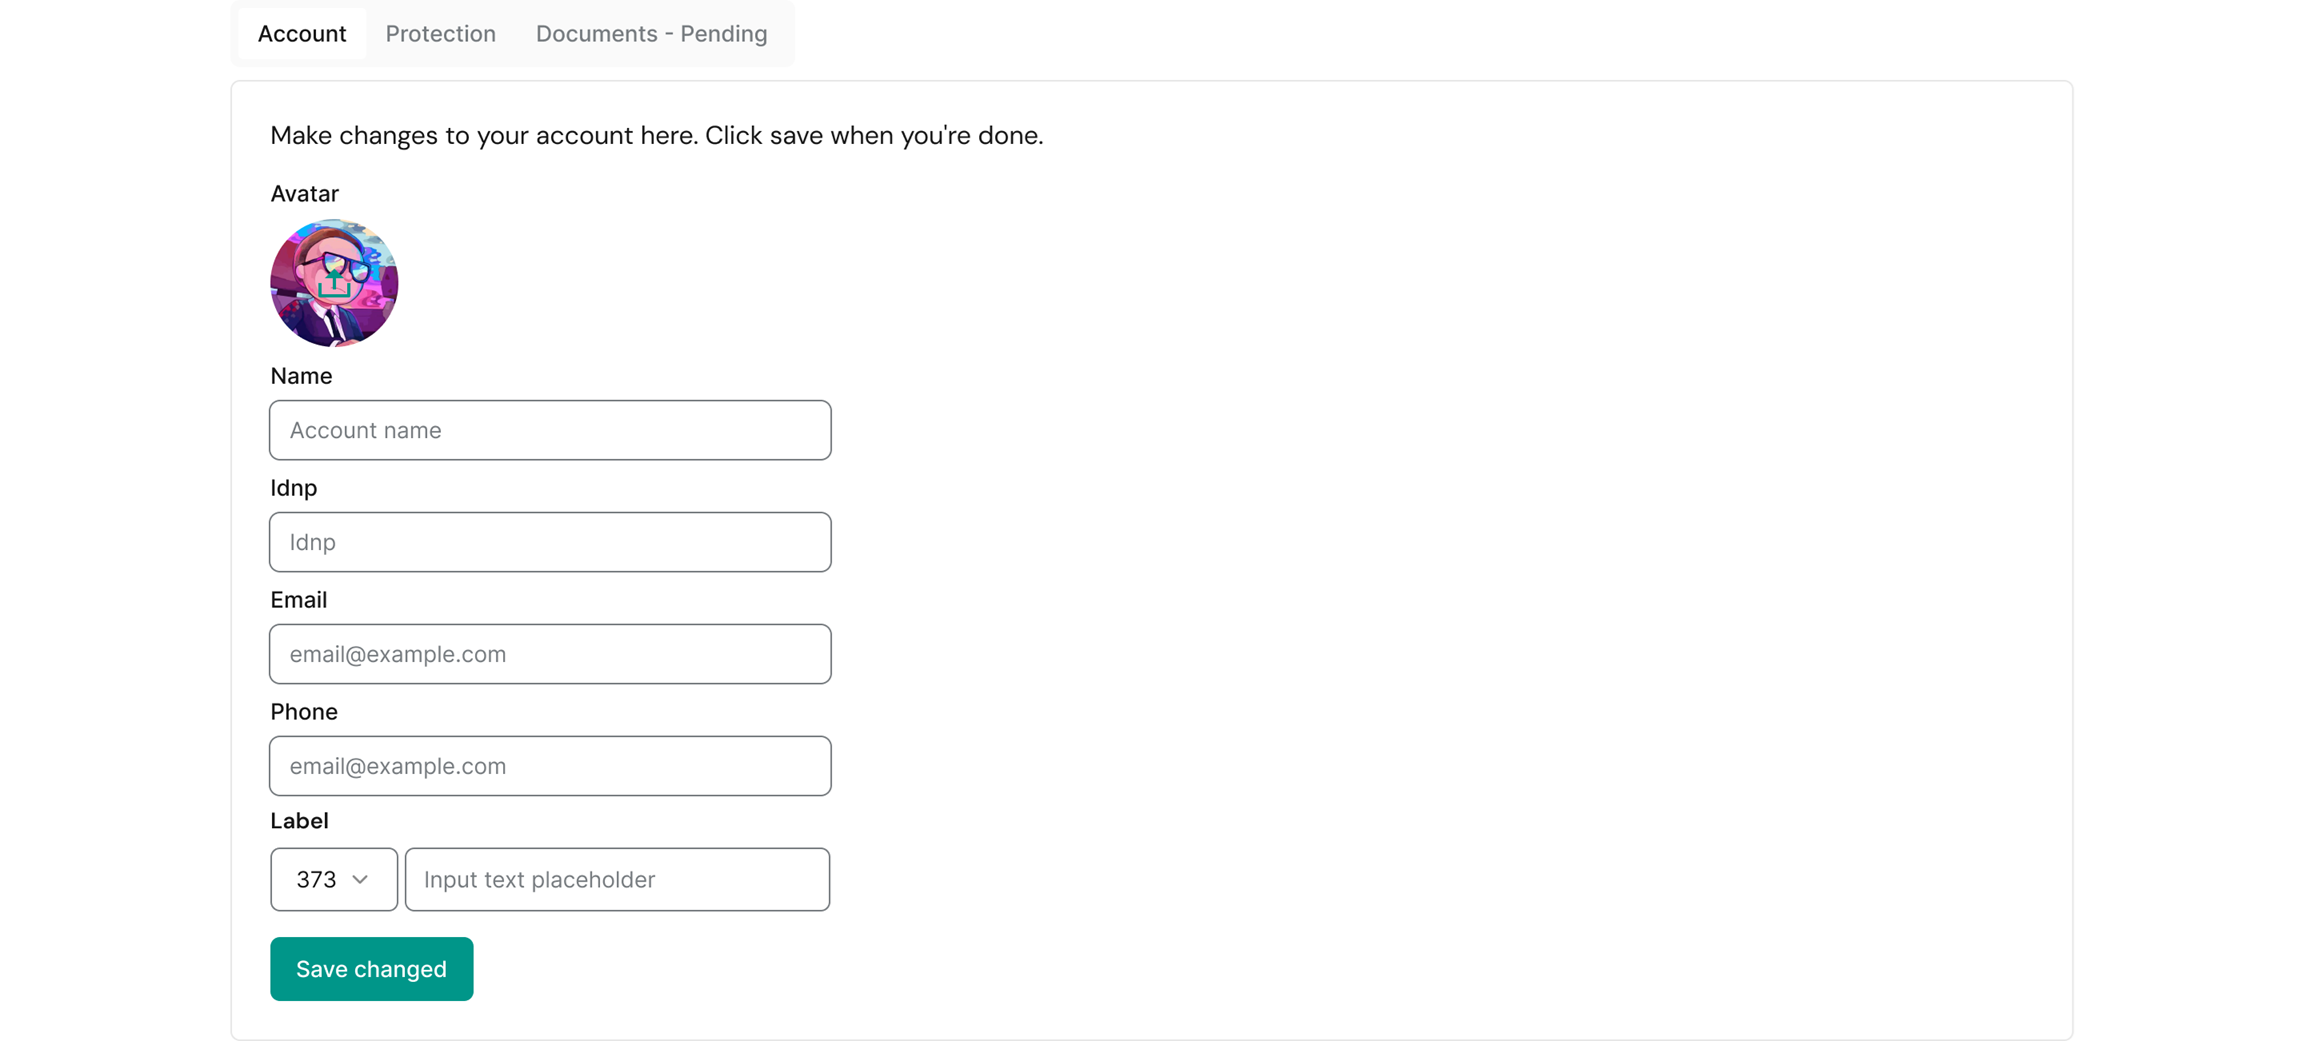
\includegraphics[width=18cm]{"images/figmaUI/accountspage-account-crop.png"}
    \caption{Account page - Possibility to modify personal info}
    \label{accountspage-account}
\end{figure}


The protection tab (Figure \ref{accountspage-protection}) provides the possibility to change password and enable multi-factor authentication.


\begin{figure}[H]
    \centering
    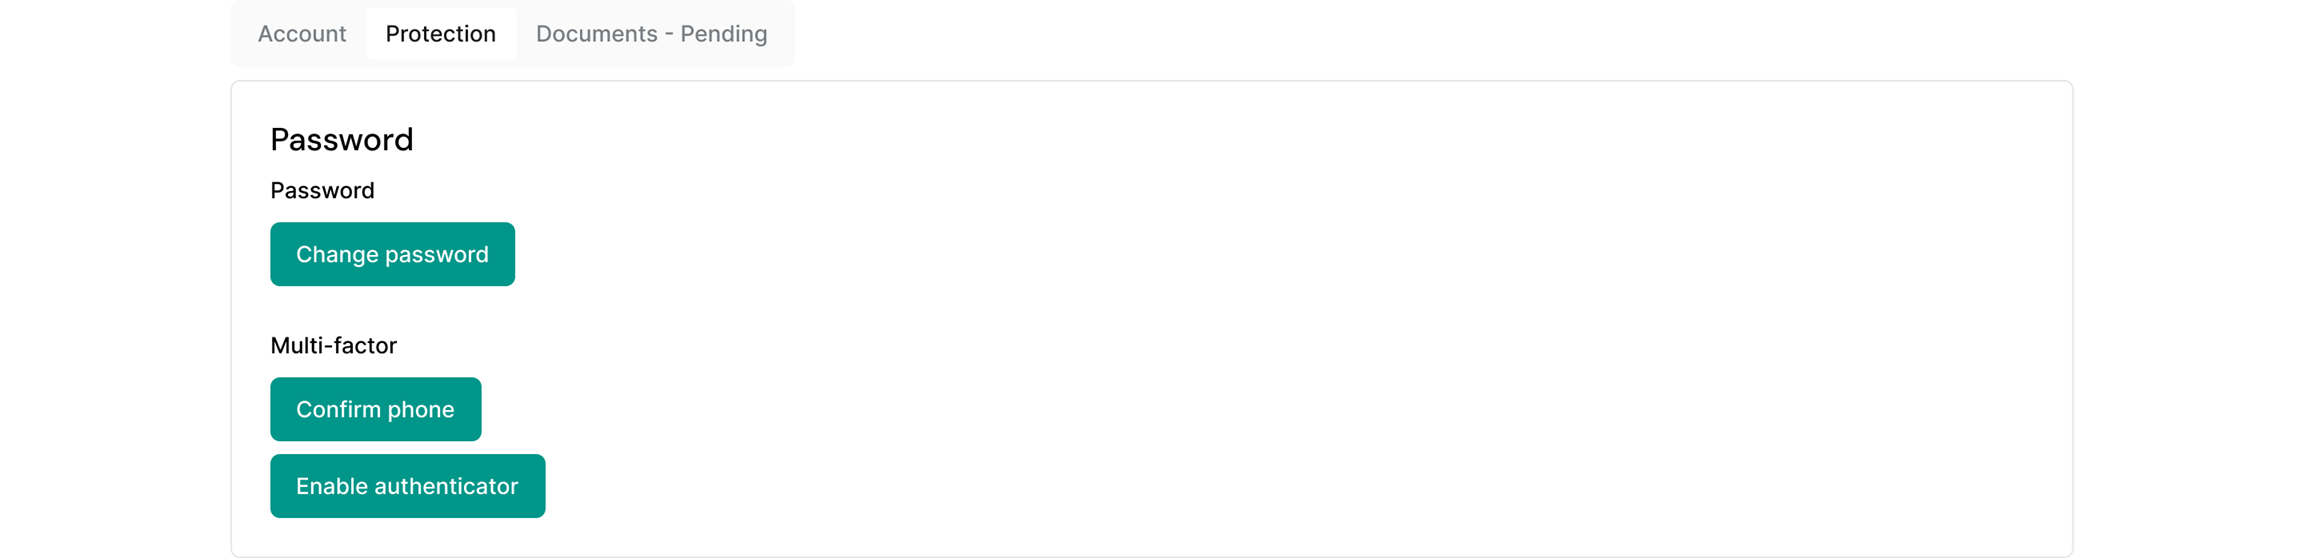
\includegraphics[width=18cm]{"images/figmaUI/accountspage-protection-crop.png"}
    \caption{Account page - Possibility to modify the protection methods}
    \label{accountspage-protection}
\end{figure}

\newpage
The documents tab (Figure \ref{accountspage-documents}) gives the user list of the documents and pending.


\begin{figure}[H]
    \centering
    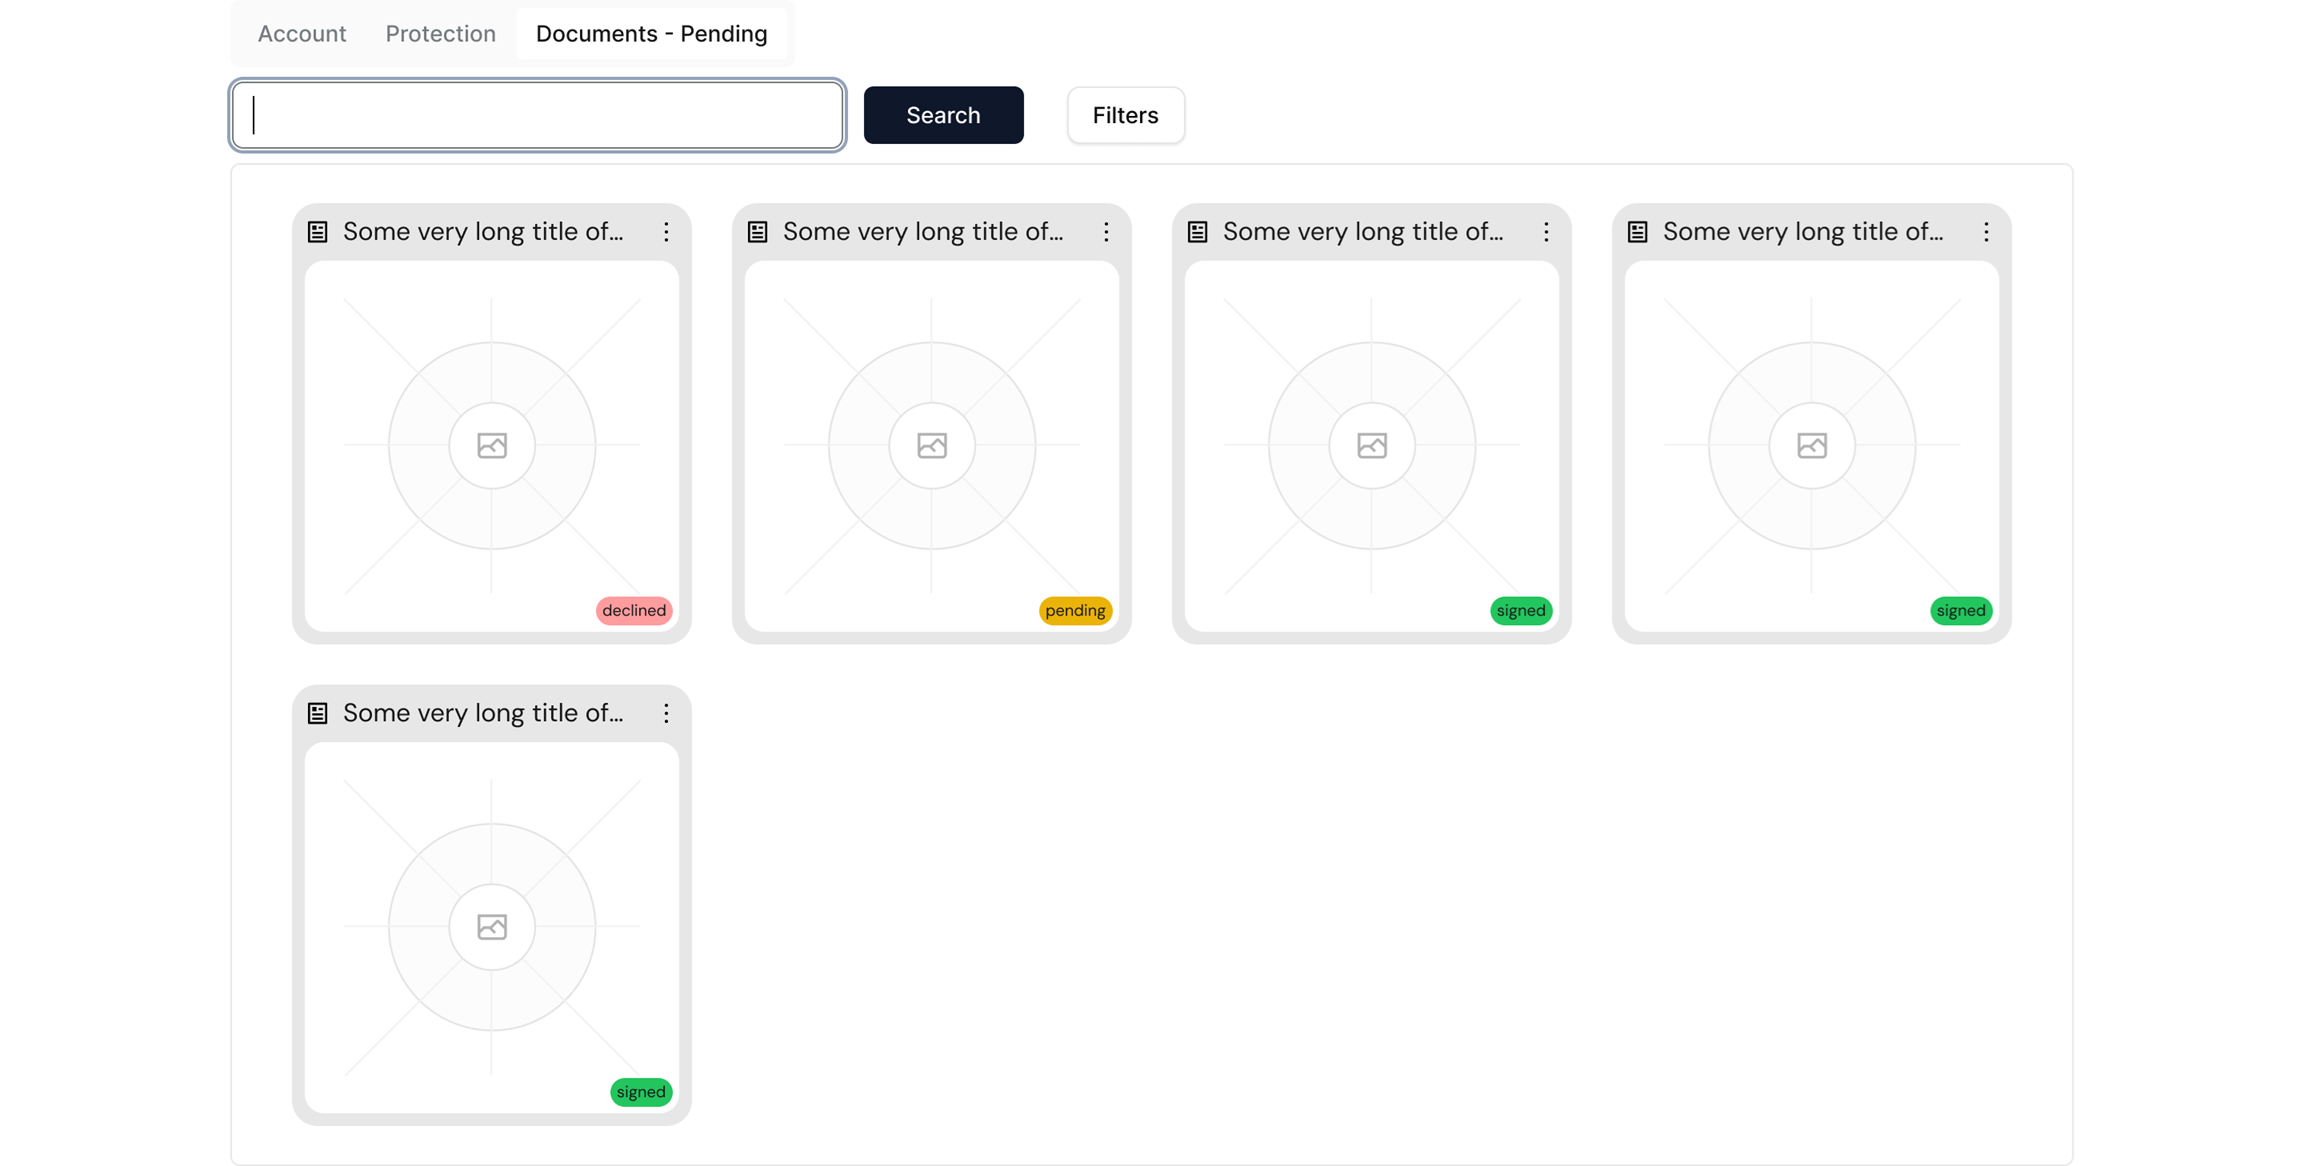
\includegraphics[width=18cm]{"images/figmaUI/accountspage-documents-crop.png"}
    \caption{Account page - View of the documents}
    \label{accountspage-documents}
\end{figure}



